\documentclass[11pt]{article}
\date{\vspace{-10ex}}

\usepackage{lineno,hyperref}
\modulolinenumbers[5]

%%%%%%%%%%%%%%%%%%%%%%%%%%%%%%%%%%%%%%%%%%%%%%%%%%%%%%%%%%%%%%%%%%%%%%%%%%
% Added lines by Gustavo Quintana to facilitate internal review process
\usepackage{amsmath, amsfonts, mathtools, hyperref, tikz, pgf, subcaption, mathdots}
\usepackage[a4paper, total={6.5in, 9in}]{geometry}
\usepackage{setspace}
\usetikzlibrary{shapes, arrows, calc, patterns, decorations.pathmorphing, decorations.markings, positioning, external}
\tikzexternalize
\tikzset{external/system call={pdflatex \tikzexternalcheckshellescape -halt-on-error -interaction=batchmode -jobname "\image" "\texsource" && pdftops -eps "\image.pdf"}}
\tikzexternalize[shell escape=-enable-write18]
\usepackage{algorithm, algorithmic, bm}
%\usepackage[noend]{algpseudocode}
\renewcommand{\algorithmicrequire}{\textbf{Input:}}
\renewcommand{\algorithmicensure}{\textbf{Output:}}
%\renewcommand{\algorithmicreturn}{\textbf{Initialize:}}

\makeatletter
\newcommand*\rel@kern[1]{\kern#1\dimexpr\macc@kerna}
\newcommand*\widebar[1]{%
  \begingroup
  \def\mathaccent##1##2{%
    \rel@kern{0.8}%
    \overline{\rel@kern{-0.8}\macc@nucleus\rel@kern{0.2}}%
    \rel@kern{-0.2}%
  }%
  \macc@depth\@ne
  \let\math@bgroup\@empty \let\math@egroup\macc@set@skewchar
  \mathsurround\z@ \frozen@everymath{\mathgroup\macc@group\relax}%
  \macc@set@skewchar\relax
  \let\mathaccentV\macc@nested@a
  \macc@nested@a\relax111{#1}%
  \endgroup
}
\makeatother
%%%%%%%%%%%%%%%%%%%%%%%%%%%%%%%%%%%%%%%%%%%%%%%%%%%%%%%%%%%%%%%%%%%%%%%%%%

%% `Elsevier LaTeX' style
\bibliographystyle{elsarticle-num}
%%%%%%%%%%%%%%%%%%%%%%%

\newtheorem{innercustomgeneric}{\customgenericname}
\providecommand{\customgenericname}{}
\newcommand{\newcustomtheorem}[2]{%
  \newenvironment{#1}[1]
  {%
   \renewcommand\customgenericname{#2}%
   \renewcommand\theinnercustomgeneric{##1}%
   \innercustomgeneric
  }
  {\endinnercustomgeneric}
}
\newcustomtheorem{customthm}{Theorem}
\newcustomtheorem{customlemma}{Lemma}

\DeclareMathAlphabet\mathbfcal{OMS}{cmsy}{b}{n}

\begin{document}


\title{Jury members' comments on the private PhD defense of \linebreak Gustavo Quintana-Carapia} 

\maketitle

Thank you to the jury members for reviewing the thesis manuscript and for giving suggestions for improvement. 
The manuscript changes due to the comments are highlighted in \color{blue} blue fontcolor\color{black}.

\section*{General comments}

\begin{itemize}
	\item The manuscript text should better position the PhD to related work. Improve the literature review and discuss (and cite) the state of the art.
	
	{\bfseries The introduction of the chapters now includes the state of the art to position the PhD work with respect to the literature.}
	
	\item  Add more clearly the motivation for the PhD research work by including motivational examples to the introduction.
	
	{\bfseries Motivational examples have been added to the Introduction. }
	
	\item  Add a discussion with comparison of existing EIV methods. Give, with the positive and negative aspects in mind, a better justification for why you use a (R)LS method, and not, e.g., (R)IV method.
	
	{\bfseries In Section 4.1.4, a discussion that compares IV methods with EIV methods has been added.}

	\item  Discuss more clearly the aspects of scalability of the methods and their limitations in terms of model order, size of data sets (e.g., related to the inversion of LS matrices).
	
	{\bfseries In Section 3.2 was added a discussion on the scalability of the data-driven step input estimation method.}
	
	\item  The equations on pages 12 and 13 seemingly contain errors and should be corrected.
	
	{\bfseries The equations on pages 12 and 13 have been corrected.}
	
	\item  The figure shown on page 66 was made with a single experiment; it is desirable to see the (averaged) effect on several experiments.
	
	{\bfseries A series of 100 runs of the maximum-likelihod estimation method has been simulated and the results have been added to the manuscript in Section 6.3.2.}
	
\end{itemize}

\section*{Lyudmila Mihaylova}

\begin{itemize}
	\item You develop results for uncertainty quantification; what type of uncertainties can your approach deal with and which levels of noise can you consider? Elaborate on SNR levels; I’m also very interested in scalability, so how big the matrices can be.
	
	{\bfseries A numerical sensitivity analysis was conducted on both subspace and maximum-likelihood methods for solving the affine input estimation problem. The sensitivity analysis showed that the subspace method can handle uncertainty on the generating system parameters up to 5\% without afecting deeply the performance of the method. Moreover, the mean-squared error of the estimation computed by the subspace method is similar in up to one order of magnitude in the SNR interval from 20 to 60 dB, being $10^{-1} \ \mathrm{g}^2$ its maximum value at 40 dB. The levels of measurement noise in practical applications are found in this SNR interval. }
	
	\item  Concerning the scalability to data: eqn 3.6: how scalable is the approach in all aspects (order, data, linked to inversion for LS matrix); can you deal with hundreds, thousands of data?
	
	{\bfseries The following paragraph has been added in Section 3.2 to discuss the scalability of the data-driven step input estimation method.}
	
	\color{blue}
    The computational complexity of the RLS algorithm solution to the system of equations (3.14) is $O \left( \left( n+1 \right)^2 \right)$.
    The largest computational requirement is for the initialization of the algorithm, where a matrix inverse is required when the number of samples is just enough to have a square matrix $\widetilde{\mathbf{K}}_{n+1}$.
    From there on, the RLS algorithm updates the solution with linear complexity.
    Therefore, even though a large number of samples $N$ makes the matrix in the system of equations (3.14) increase in the number of rows, the estimation of the solution does not increase in complexity. 
    The data-driven step input estimation method is then scalable for any sensor of order $n$, and can be executed in devices with limited computational resources, provided that the computation of the  $n+1 \times n+1$ inverse matrix is feasible.
    \color{black}	
	
	\item  What recommendation up to scale/order can method work with. What are the limitations? It would be good to have more precise discussion about these aspects in dissertation: what do you mean by large scalability: 100, $10^4$, ...? A more detailed discussion is desirable.
	
	{\bfseries In Section 3.2 was added a discussion on the scalability of the data-driven step input estimation method. Since it uses recursive least squares to update the estimation, its complexity is linear in the number of parameters $n+1$. This means that for small number of samples, $N=100$, or large number os samples, $N=10^4$, the complexity per recursion does not change.
	
	The computation of the bias and variance of the input estimation, as it is proposed in Chapter 4, has a complexity $O(n^3N)$. This complexity prevents the implementation in real time of these statistical moments estimation. A future research work can be devoted to find efficient estimation of these input estimation moments, to be obtained right after the input estimation itself. }
	
	\item  On slide 25 (noisy graphs) it would be good to see a statistical analysis (more experiments than one).
	
    {\bfseries 100 runs of the maximum-likelihod estimation method have been simulated and their results have been added to the manuscript in Section 6.3.2.}
	
	\color{blue} 
    The maximum-likelihood (ML) method estimated the affine input parameters from the sensor model transient response.
    A total of 100 runs of the method were obtained, using different realizations of measurement noise.
    The measurement noise variance was set to have an SNR of 40 dB.
    The ML method used the first 50 samples to initialize the optimization variables and updated the variables every $N_{\mathrm{s}} = 5$ samples.
    Figure \ref{fig:rele_lo_40dB_s10} shows the average of the observed relative errors in the estimation of the parameters $\widehat{a}$, $\widehat{b}$, $\widehat{x}_{\mathrm{ini,1}}$, and $\widehat{x}_{\mathrm{ini,2}}$.
    
    \renewcommand{\thefigure}{6.8}
    \begin{figure}[!htbp]
    \centering
    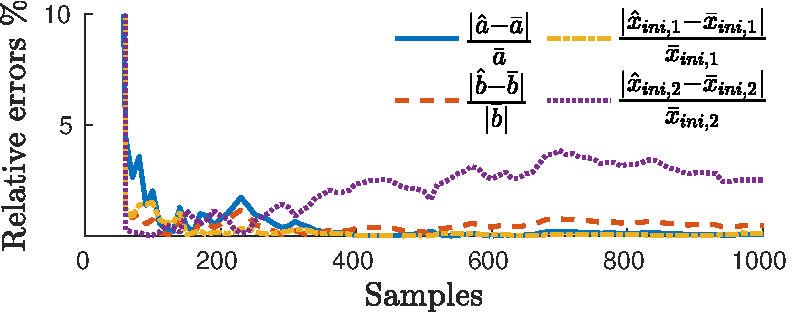
\includegraphics[width=0.6\columnwidth]{../ChapterRampInput/fig/Fig_7.pdf} 
    \caption{ \label{fig:rele_lo_40dB_s10} The affine input parameters and the sensor's initial conditions are estimated with the ML method. After three iterations, \color{blue} the average of the relative error is smaller than 5 \% for each and every of the estimates. The estimate $\widehat{x}_{\mathrm{ini,2}}$ has the larger relative error near to 1 \%. \color{black} }
    \end{figure}

    Figure \ref{fig:cov_lo_40dB_s1} shows \color{blue} the average \color{black} of the variances that were observed on the diagonal of the covariance matrix $\mathbf{J}$. 
    We can see that the estimation variances decrease as more samples are processed.
    Moreover, the estimation variances of $\widehat{a}$ and $\widehat{b}$ obtained with the ML method are lower than the corresponding estimation MSE errors obtained from a Monte Carlo simulation of the subspace method.

    \renewcommand{\thefigure}{6.9}
    \begin{figure}[!htbp]
    \centering
    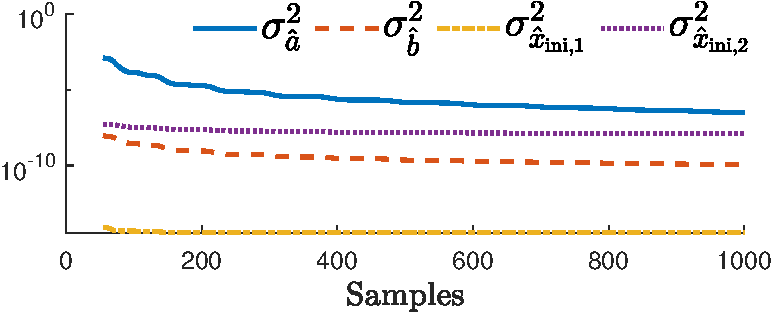
\includegraphics[width=0.6\columnwidth]{../ChapterRampInput/fig/Fig_8.pdf} 
    \caption{ \label{fig:cov_lo_40dB_s1} The variances of the ML estimates are calculated using the information provided by the analytic Jacobian. \color{blue} The estimates $\widehat{x}_{\mathrm{ini,1}}$ and $\widehat{a}$ have the smaller and larger variances, respectively. \color{black}  }
    \end{figure}

    \color{black} 

\end{itemize}

\section*{Stephane Chretien}

\begin{itemize}
	\item The Taylor expansion is computed of order 2, what is the accuracy of expansion with respect to system, noise level,... Can you come up with a priori bound on error that will allow you to assess the quality of the expansion? Can you predict where the solution is going to be before computing Taylor expansion?
	
	{\bfseries An a priori bound on the error introduced by the Taylor series expansion can be obtained in terms of the spectral radius of the matrix $\mathbf{M}$. In Section 4.1 the following description has been added: }
	
    \color{blue} An a priori bound on the error introduced by the second order Taylor series expansion can be expressed in terms of the spectral radius $\rho(\mathbf{M})$.
    Considering that the Taylor series expansion is an infinite sum we have that
    \begin{equation} \tag{4.4} \begin{aligned} (\mathbf{I} + \mathbf{M})^{-1} &= \mathbf{I} - \mathbf{M} + \mathbf{M}^2 - \mathbf{M}^3 + \ldots \\
    &=  \mathbf{I} - \mathbf{M} + \mathbf{M}^2 - \mathbf{M}^3 \left( \mathbf{I} - \mathbf{M} + \mathbf{M}^2 - \mathbf{M}^3 + \ldots \right) \\
    &=  \mathbf{I} - \mathbf{M} + \mathbf{M}^2 - \mathbf{M}^3  (\mathbf{I} + \mathbf{M})^{-1} \end{aligned} \end{equation} 
    Therefore we can obtain a bound for the second error expansion error if we take a matrix norm as follows
    \begin{equation} \tag{4.5} \begin{aligned} \| (\mathbf{I} + \mathbf{M})^{-1} - ( \mathbf{I} - \mathbf{M} + \mathbf{M}^2 ) \| &=  \| \mathbf{M}^3  (\mathbf{I} + \mathbf{M})^{-1} \| \\
    & \leq \| \mathbf{M}^3 \| \| (\mathbf{I} + \mathbf{M})^{-1} \| \leq \dfrac{\| \mathbf{M} \|^3}{ 1 -  \| \mathbf{M} \|} = \dfrac{\rho(\mathbf{M})^3}{1 - \rho(\mathbf{M})}  \end{aligned} \end{equation} 
	\color{black}
	
	\item  Concerning other sorts of prior estimations, e.g., given by explicit function theorems. I wonder if you could get something and apply this bound in order to control the bound of the 2nd order expansion. There exist some good results that could help you devise something a priori which can control the error you are making. Neuberger's results (quite old now) but may be handy for this kind of problem. This can be investigated further.
	
	{\bfseries The investigation of the error bounds for the second order Taylor expansion can be conducted using the continuous Newton method. This is proposed as future research work in Chapter 7.}
	
	\color{blue}
	Neuberger's paper \cite{Neuberger07} introduces five theorems that are consequence of the continuous Newton method.
	The Newton method aims to find a zero of the function $F: R^n \rightarrow R^n$ by iterating
	\begin{equation} z_{k+1} = z_k - \left(F' (z_k) \right)^{-1} F(z_k) \end{equation}
	for $k=0,1,2,\ldots$, and for a given initial $z_0$, assuming that $\left(F' (y) \right)^{-1}$ exists for some $y \in R^n$.
	A domain of attraction is the set of all initial values $z_0$ that lead to a root of $F$ after the convergence $z_0, z_1, z_2,\ldots$.
	The damped Newton method  
	\begin{equation} z_{k+1} = z_k - \delta_k \left(F' (z_k) \right)^{-1} F(z_k) \end{equation}
	prevents convergence issues, such as chaotic domains of attraction, with $\delta_1, \delta_2, \ldots \in (0, 1)$. 
	The continuous Newton method is a sequence of damped Newton methods. To implement the continuous Newton method, select $0<T<1$ and perfom $m$ runs of the damped Newton method with $\delta_k = T/m$, for $k=1,2,\ldots, m$.
	The result $z_{k+1}$ is the zero estimation $x_m$, and if the sequence of estimates $x_1, x_2, \ldots$ converges, then it converges to the result of the continuous Newton method.
	
	The objective of the continuous Newton method is to find a function $z: [0, \infty) \rightarrow R^n$, so that
    \begin{equation} z(0) = x \in R^n, \quad z' (t) = - \left(F' (z(t)) \right)^{-1} F(z(t)), \quad t \geq 0, \label{eqn:contNewton}\end{equation}
    subject to the existence of the limit $u=\mathrm{lim}_{t \rightarrow \infty}{z(t)}$, that satisfies $F(u)=0$.
    This implies 
    \begin{equation}  F' (z(t)) z' (t) = - F(z(t)) , \end{equation}
    that is equivalent to
    \begin{equation}  \left(F \circ z\right)' (t) = - F(z(t)) , \end{equation}
    from where we get
    \begin{equation}  F(z(t)) = e^{-t} F(z(0)) . \end{equation}
    Thus, the residual $F(z(t))$ only changes in magnitude and not in direction.
    This property is essential for the results of the theorems in \cite{Neuberger07}. 
    In particular, Theorem 5 gives the conditions for the continuous Newton method to ensure finding a root of the function.
    
    \begin{customthm}{5} \label{thm:five}
    Suppose that each of $H$, $J$, and $K$ is a Banach space, with $H$ compactly embedded in $J$, that $r>0$, and that $G:B_r(0) \rightarrow K$ is continuous as a function on $J$. Suppose also that $g$ belongs to $K$ and that for each $y$ in $b_r(0)$ there is an $h$ in $B_r(0)$, where $b_r(0)$ and $B_r(0)$ are open and closed balls in $H$ of radius $r$ centered at 0, such that
    \begin{equation} \lim\limits_{t \to 0+} -{\dfrac{1}{t} \left(G(y+th) - G(y)\right) = g}. \end{equation}
    Then, there exists $u$ in $B_r(0)$ such that $G(u)=g$.
    \end{customthm}
    %$F:B_r(0) \rightarrow K$
    
    The theorem implies that $u$ is a zero of the function  defined as $F(y) = G(y) - g$.  
    Since $G$ is a continuous function and if $\left(G' (y) \right)^{-1}$ exists for each $y$ in $B_r(0)$, a metric for the validity of the Theorem (\ref{thm:five}) hypothesis is the inequality $\left\Vert  \left( G' (y) \right)^{-1} g \right\Vert \leq r$.
    
    To link the data-driven step-input estimation problem with this theorem, we can take the system of linear equations $\widetilde{\mathbf{y}} = \widetilde{\mathbf{K}} \bm{\theta}$, then define $G(y) = \widetilde{\mathbf{K}} \bm{\theta}$, and $g = \widetilde{\mathbf{y}}$, so that we have $F(\bm{\theta}) = G(\bm{\theta}) - g$. The derivative of the function $G(\bm{\theta})$ is given by $G'(\bm{\theta}) = \widetilde{\mathbf{K}} \mathbf{I}$. Using the pseudo-inverse of $\widetilde{\mathbf{K}}$, the metric $\left\Vert  \widetilde{\mathbf{K}}^{\dagger} \widetilde{\mathbf{y}} \right\Vert \leq r$ indicates that the estimate $\hat{\bm{\theta}}$ is found inside a ball of radius $r$.
    The questions that remain open are how large can $r$ be?, and how is the radius $r$ related to the perturbation noise variance? 
	\color{black}
	
	\item  About trying to find a good transformation from LS to EIV model. I am wondering if you can think of other more accurate starting points instead of LS. Closer to the problem you want to study, but still preserving computational lightness? The closer you start from objective, better the Taylor expansion would be.. Something to investigate as well...
	
	{\bfseries To get starting points to the EIV model, that are more accurate than LS, we would need to incorporate more prior knowledge. In the formulation of the EIV problem we have made assumptions of the model class for the sensor and the Gaussian white noise of given variance for the additive measurement noise. The LS is an heuristic algorithm that was chosen by its simplicity for solving online the estimation problem by means of recursion. However, the LS solution is biased. The optimal solution could be obtained with a maximum likelihood algorithm provided we have a large amount of samples, but we need to provide approximations starting from small number of samples. Moreover, the maximum likelihood solution of the EIV problem needs structured total least squares, which does not have a closed form that could be extended with a Taylor series, or structured total maximum likelihood, which do not support the correlation between the regression matrix and the regressor in the EIV problem. The recursive versions of these two structured approaches is also more computational expensive than RLS. Therefore, it is required to continue the research towards efficient solution algorithms.  }
	
	\item  About robustness: is it an issue in practical problems with heavy tailed noise, outliers,... Perhaps the use of median of means plugged into your approach might produce interesting alternatives for outliers or heavy tailed data. But this is an intricate thing to deal with. Might be interesting to ponder this in future.
	
	{\bfseries There are some estimators that can deal with heavy tailed noise. In the paper \cite{Balkema18} there  are described different estimators for a linear regression \linebreak $Y_i = b+a X_i + Y_i^{*}, \quad i = 1,\ldots,n$, where both the explanatory variables $X_i$ and the errors $Y_i^{*}$ have heavy tails. The $X_i$ are samples from a Pareto distribution on $(1, \infty)$ arranged in decreasing order $X_n<\cdots<X_2<X_1$, as if they were generated from the order statistics $U_1<\cdots<U_n$ of a sample of uniform variables in $(0,1)$ by setting $X_i = 1/U_i^\zeta$. The parameter $\zeta$ is the tail index of the Pareto distribution. For the variables $Y_i^*$, the tail index is $\eta$. 
	Heavy tails are indicated by larger tail indexes. For $\eta < 1/2$, the variable $Y^*$ has finite variance and least squares is the suggested estimator. For $\zeta < 1/2$, the variable $X$ has finite variance and the least absolute deviation is the suggested estimator, otherwise the Theil-Sen estimator is preferable. The paper presents empirical results comparing the estimation bias and standard deviation for different tail indexes.
		
	Regarding outliers, in \cite{Maronna06} is described an approach of using least squares to identify the outliers, followed by a recalculation without considering the outliers. In this sense, one could also consider that the removed outliers are missing data, and use low-rank approximation. The classical approach is using a maximum likelihood type estimator (M-estimators) as it is described in \cite{Zhang97} and \cite{Huber81}. The M-estimators aim to mitigate the outliers impact by using a function of the residual $\rho(r_i)$ instead of the the squared residuals $r_i^2$ in the minimization $\text{min} \ \sum{\rho(r_i)}$. The function $\rho$ is symmetric, positive definite, with only one minimum at 0, and increasing slowly than the the square.  
	
	Selecting another estimator to solve the EIV problem constructed by the data-driven step input estimation problem to deal with heavy tailed noise, or with outliers, might have a big impact on the implementation. The implementation may be computationally complex and not suitable for online applications.  

	
	
	
	}
	
	\item  On deep learning: could this be an alternative?
	
	{\bfseries Deep learning could be used but it would be an overkill methodology for linear estimation. However, for metrology applications were the input is the to-be-estimated signal, implementing deep learning could be a challenge. The neural networks are suitable for non-linear model based applications were the training require the design and application of input stimuli to correlate with the corresponding outputs of the system. 
	In metrology, it is not possible to train deep learning methodologies with real input data, because the input data is unknown and cannot be observed. 
	By applying neural networks trained by simulation would estimate inaccurately the desired inputs.  }
	
	
\end{itemize}

\section*{Guillaume Mercere}

\begin{itemize}
	\item In the first or second sentence: “users cannot wait for a steady state regime” . Do you have specific examples of real industrial systems for which it is necessary to have continuous read-out before steady-state is reached? - Further on the industrial part and selling sensors with data-driven parts. Can you explain to experts that your solution is better? Sensors will be used for ages; why not spend one day to do system identification and get a reliable model to make a compensator, instead of using your approach?
	
	{\bfseries The fast weighing of parcels in the post office is a typical example of the real life systems where the time is limited to perform the measurements. Another one that we see nowadays is the temperature measurement of people in airports or train stations to prevent the spread of corona virus. The data driven method can be implemented in portable devices with limited computational resources. In industrial plants were a time slot can be devoted to identify the measurement system and implement a compensation method, the solution might be useful only for a certain amount of time. It is assumed that the model approximation deviates due to changes in the system elements, leading to inaccuracies in the inpiut estimation. There is a need for adaptive methods to avoid stopping the production lines to repeat the system identification procedure. The data-driven method is such an adaptive method. }
	
	\item  Chapter 2, Section 2.2.1. Can you give me some classic solutions/algorithms instead of LS in general? (Say I'm not familiar with EIV or TLS?) Usually with LS problems: multiply with $K^\top$ and compute pseudoinverse. Do you know another solution where they don't use K on the left-hand-side but something else? To get rid of noise by using a matrix on the left-hand-side, is related to EIV. There are some recursive solutions for this. It could be interesting to compare with such IV solutions.
	
	{\bfseries In Section 2.2.1 the follwing paragraphs have been modified to include references of instrumental variable solutions to the errors-in-variables problems.}
	
	\color{blue}
	Instead of using a total least-squares (TLS), or an intrumental variables, solution of the structured EIV problem, the step input estimation method uses the recursive least-squares solution (RLS). 
    In the review conducted by \cite{Markovsky07overview} it is shown that the TLS solution of unstructured EIV problems is consistent when the perturbations have zero mean with a given positive definite covariance, and
    the TLS solution is equivalent to the maximum likelihood (ML) solution when the disturbances of the EIV problems are i.i.d. normally distributed. 
    The classical TLS solution is obtained using singular value decomposition of the augmented matrix built from the regression matrix and the regressor as additional columns.
    However, the studies presented in \cite{VanHuffel07TLSeditorial} demonstrate that the structured TLS solutions cannot be generalized since each structure in an EIV problem requires a specific treatment. 
    Moreover, the ML estimator of structured EIV problems leads to non-convex optimization, and the global optimum is not guaranteed \cite{Beck10}.
    On the other hand, the instrumental variable (IV) solution of EIV problems use an additional variable.
    The additional variable is an instrument with the purpose of improving the consistency of the estimate.
    To do this, the construction of the instrumental variable has to be done in such a way that it is uncorrelated with the perturbations and correlated with the regressor, as it is described in \cite{Soderstrom18}. 
    Unfortunately, the computational complexity of the TLS, ML, and IV solutions inhibits their real-time implementation.

    The solution of the step input estimation problem is preferred to be online, since its applications are in the field of metrology.
    In the literature there are references for online implementations of TLS, ML or IV methods, which are are mainly recursive versions of the solution methods.
    These recursive versions are developed to solve EIV problems for system identification and fault detection.
    We have, for example, generalized recursive TLS solutions introduced in \cite{Rhode14recursive} and \cite{Rhode14recursivecov}, and recursive IV solutions developed in \cite{Djouambi12}, \cite{Shang16} and \cite{Gil15}.
    These methods cannot be used as off-the-shelf solutions to the step input estimation EIV problem because they require to be adapted to the specific requirements of the problem.
    One is that the sensor output is the only measured signal, since the input is to-be estimated, and the solution should be simpler, preferable with a linear complexity $O(n)$, instead of the cubic $O(n^3)$ or cuadratic $O(n^2)$ complexities of the mentioned recursive methods, where $n$ is the sensor order.
    The proposal of the data-driven step input estimation method includes the recursive least-squares (RLS) solution.
    Compared to recursive TLS or recursive IV solutions, RLS is suboptimal but more simple solution to the structured EIV problem with lower computational complexity,  suitable for real-time implementation.
	\color{black}

	
	\item  In Chapter 3: at beginning you say to use linear systems theory to model a sensor. Can you discuss this assumption: is it true in practice? Can you guarantee it behaves like an LTI system?
	
	{\bfseries The first paragraph of Chapter 3 has been added to explain this concept:  }
	
	\color{blue}
    The dynamic systems in the real world are non linear. 
    Under certain intervals of operation, the linear approximations can explain the dynamics of the systems. 
    The linear and time invariant systems have been studied in depth and the linear theory is a solid collection of tools to analyze and explain the behaviour of dynamic systems in a wide range of applications. 
    On the other hand, the study of non-linear systems is more complex and strongly depends on the type of non-linearity that each particular systems exhibit. 
    When the non-linear modeling does not apport a big amount of benefits into the application study, such as significative accuracy improvement or supporting wide ranges of operation, then is better to resort to the utilization of LTI representations. 
    A sensor is a dynamic system whose operation range is preferred to be linear, to facilitate the repeatability and reproducibility of the measurements.
    This means that every time the sensor must deliver identical responses for the same input excitations.   
    \color{black}

	\item  Equation 3.1: an LTI system, described with SS representation. You only put output noise on this representation. People sometimes also add process noise. Why? How to modify your approach if there is process noise? Is it still white in this case?
	
	{\bfseries In Chapter 3 was added the following paragraph to explain the impact of white process noise in the response of al LTI system. }
	
	\color{blue} 
    The process noise is the representation of the uncertainty in the system state due to unmodeled perturbations that affect the state evolution. 
    The process noise is modeled as an additional input to the system excitation. 
    For a linear time invariant (LTI) system, the response to a sum of two input excitations is the sum of the two responses that correspond to the individual inputs.
    It is demonstrated in \cite{Gubner06} and \cite{Smith11} that the response of an LTI system to a white noise input is colored noise, since the power spectral density of the response is not constant, but instead proportional to the squared magnitude of the system impulse response.
    Nevertheless, in the bandwidth operation of a properly designed measurement system, processing white noise results in approximately white noise output. 
    Moreover, in the present work the measurement noise exists only in the system response signal, because the input is not direcly observed, and the sensor operation is not subject to external perturbation. 
    Under these conditions, the mean and variance of the measurement noise $\epsilon$ describe implicitly the process noise entering the system. 
    \color{black}

	\item  On page 12 standard approach top of page equation: there are some mistakes in the equations! there is no epsilon (noise) in the equation. But then you do an SVD of H and estimate from there. How does it work if you have noise? Have you tried implementing it and see what you get?
	
	{\bfseries The step input estimation based on singular value decomposition works only with exact data. When  noise perturbes the sensor response the method cannot guarantee the step input estimation. The singular value decomposition of a Hankel matrix constructed from a perturbed sensor response provides only an approximation of the singular values and the singular vectors of this Hankel matrix. Then, the step input estimation obtained with this method from perturbed sensor response is only a rough estimation.     }
	
	\item  On page 12: I’m not sure the equations at the end of the page are correct, e.g., Y=G ubar ... not sure there is x; same for rest; There seem to be many mistakes here and next pages. Be careful with the equations!
	
	{\bfseries The equations have been reviewed and the typos were corrected.}
	
	\item  On page 13, you assume persistency of excitation of order $L$. How do you check this? In your case the input is constant; how to guarantee that the assumption is met?
	
	{\bfseries The persistency of excitation of a signal is verified by looking at the rank of the Hankel matrix constructed from the consecutive samples of this signal. When the Hankel matrix of $L+1$ block rows has a rank lower or equal than L, then we say that the signal is persistently exciting of order $L$. A step input has a very low order of persistency $L=1$, but the step respose of a system has a larger order of persistency. In fact, we assume that if the persistency of excitation of the step response is sufficiently high, then the columns of the Hankel matrix constructed from the step response span a linear space with all the responses of the equivalent augmented autonomous system where the step input is considered an augmented initial condition.}

	\item  In Chapter 4, p 17, Section 4.1.1: You assume that perturbations are IID and must be normally distributed. Why using an assumption of normally distributed? I would think that the kind of distribution is important for CRLB, but I’m not sure you need it for eqns 4.8, 4.9, 4.10,... IID is important, normality perhaps not.
	
	{\bfseries The following paragraph has been added in Section 4.1 to discuss on the need for the normality assumption.  }
	
	\color{blue}
	The normality assumption is necessary to provide more prior information into the method formulation.
    The second order Taylor series expansion (4.6) is developed considering the perturbation noise that gets into the regression matrix from the sensor transient response.
    Assuming only that the perturbation noise is distributed with zero mean and variance $\sigma_{\bm{\epsilon}}^2$ is not enough.
    If we additionally assume normality for the perturbation noise, then we benefit from the knowledge of the third moment equal to zero due to symmetry, and the fourth moment equal to three times the squared variance.
    \color{black}
	
	\item   In equation 4.11 you have $\sigma_eps^2 + \sigma_e^2$; how to get in practice $\sigma_e$? Do you have to do this each time? Recursively?
	
	{\bfseries The measurementy noise variance is prior information and in Chapter 5 we describe two ways of estimating $\sigma_{\bm{\epsilon}}$ In summary, the measurement noise can be extracted fom the sensor ressponse once the transient effects are smaller than the noise floor, or from the sensor response power spectrum. The online estimation of the measurement noise, simultaneously with the online step input estimation is a topic for future research.   }
	
	
	\item   Switch to 4.2, simulation results: first part dedicated to K, randomly generated; not sure if still possible, but in all your results it would be nice to have somewhere explicitly K = ... (even if randomly generated). You use only one realization also for matrices A, B, C, D in the text, so it can be added explicitly.
	
	{\bfseries Section 4.2 has been improved to explain how the exact data and the perturbation noise are generated. This modification allows to reproduce the simulations conducted and understand the outcome of them. }
	
	
	\item   in Fig 4.1 the bottom figure also discusses the structured case. Why do you talk about structured results in a section about the unstructured case?
	
	{\bfseries Section 4.2 has been improved to describe the result next to its discussion.  }
	
	\item   In 4.1 uses a constant K, but in 4.2.2 you use A, B, C, D, without any links to K. You compare the two curves generated from different data sets… It is strange to compare them. I don't see the link between both.
	
	{\bfseries Section 4.2 has been reestructured and the simulation for the unstructured case were redone to establish a link between the two cases. The exact data is the same in the two cases and the perturbation noise follows the corresponding rules of each case, with the same variance noise levels. In this way the comparison between the two cases makes more sense.  }
	
	\item To show comparison between structured and unstructured case, use unstructured results for structured case; then use unstructured results for structured case and cover all the possibilities. Now you compare curves related to two different simulations.
		
	{\bfseries The numerical study of the expressions that calculate the step input estimation bias and variance has been appended to include the results of using unstructured perturbation in the expressions for the structured case, and also structured perturbation in the expressions for the unstructured case. It is expected that the performance is very far from that obtained when using the expressions in concordance with the type data they were derived for. A discussion on this observations is included in Section 4.2.3.}
	
	\item   I was surprised to read in Chapter 5 something very close to what I read in chapter 4. In both cases generated A, B, C. In 5.1 again oscillating 5th order system, similar conclusions, ... What is the added value of 5.1 wrt 4.2.2?
	
	{\bfseries The derivation described in Chapter 4 was conducted with a second order mass-spring-damper weighing system example on mind, and the results observed were submitted in the corresponding paper. Afterwards, when we moved to the practical implementation, we faced the increase of the model order after setting up the weighing experiment. The lowest order we can assume is fifth order. So we decided to repeat the simulations and these new results serve two purposes: a transition from simulation to experimental results, and also to get an insight on the impact of the bias and variance predictions after increasing the model order.    }
	
	\item   On the impact of selected order on results. You were talking about a related bias/variance trade off. So, do you know in the literature some solutions to avoid overfitting? Can you cite something? Can you use something in your case to test for a good order of system?
	
	{\bfseries If we evaluate the step input estimation bias and variance obtained by the data-driven method for different model orders, we expect the results follow the bias-variance tradeoff. It is commonly accepted that for decreasing orders the bias is large since not all dynamics are captured, and that for increasing orders the bias is small and the variance is large because the system dynamics are captured and also the measurement noise is being modeled. However, after observing the results in the experimental validation of the method, we get better performance by overfitting. This could be valid only for some estimators. 
	For example, in the research work of \cite{Neal19} it is described a neural network that does not follow the bias variance tradeoff, contradicting \cite{Geman92} and \cite{Manning08}, who state that an overparameterized neural network reduces the bias by interpolating the data with a significant variance contribution to the mean-squared error.
	
	Some approaches described in the literature to avoid overfitting include crossvalidation (CV), minimum description length (MDL) and the Akaike information criterion (AIC).
	These methodologies are described in books such as \cite{Hastie09}  and \cite{James13}. 
	In the paper \cite{Arlot10}, CV and MDL are compared trying to answer whether penalized criteria in classical AIC should be preferred to CV for a given model selection problem. 
	On one hand, provided the data is i.i.d., CV gives good model selection in almost any framework. 
	On the other hand, CV can be less accurate, even with larger computational cost, than procedures designed to be optimal in a specific framework, such as AIC.
	
	To describe the classical methods, the following paragraph has been added in subsection 5.2.
	}
	
	\color{blue}
	
	There exist methods for estimating the performance of different models that are useful to choose among the models.
	The model selection methods can be analytical, such as the Akaike information criterion (AIC) introduced in the paper of \cite{Akaike74}, the minimum description length (MDL) iniciated by the work of \cite{Rissanen78}, or numerical such as crossvalidation.
	The AIC is defined for a class of models fit by maximum likelihood. 
	For the linear regression problem with Gaussian perturbation (3.20), the AIC is given by
	\begin{equation} \tag{5.9} \mathrm{AIC} = 2 \left( n+1 \right) - \mathrm{ln} \left( \widehat{L} \right) \label{eqn:AIC} \end{equation}
	where $n+1$ is the number of estimated parameters, and $\widehat{L}$ is the maximum value of the likelihood function of the model.
	The AIC rewards the goodness of fit by considering the maximum likelihood value, and adds a penalty term that increases the cost with respect to the number of parameters to prevent overfitting.
	In the opinion of \cite{McElreath20}, the AIC is reliable when the priors overwhelmed by the likelihood, the posterior distribution is approximately multivariate Gaussian, and the sample size is much larger than the number of parameters.
	Using this criterion for model selection is simple, \cite{Hastie09} suggest just picking the model that provides the smallest AIC value.

	The MDL approach is motivated from an optimal coding viewpoint, aiming to choose the most parsimonious model, that, according to \cite{Hastie09}, is the shortest model that can encode the data for transmision of messages.
	If we have a model with parameters $\theta$, and data $(K, y)$, with the conditional probability of the outputs $\mathrm{P}(y | \theta, K)$, and assuming the receiver knows the inputs and we transmit the outputs, then the message length required to transmit the outputs is
    \begin{equation} \tag{5.10} \mathrm{length} = - \mathrm{ln} \left( \mathrm{P}( \theta ) \right) - \mathrm{ln} \left( \mathrm{P}(y | \theta, K) \right) . \label{eqn:MDL} \end{equation}
    The length is the sum of the code length required for transmitting the model parameters with the code length required for transmitting the discrepancy between the model and the actual target values. 
    The recommended model is the one that minimizes (\ref{eqn:MDL}).
	\cite{McElreath20} arguments that model fitting is a form of data compression, where parameters explain the relationships among the data. 
	The parameters compress the data into a simpler form, with some loss of information about the sample, and 
	can be used to generate new data by decompression.
	Learning about the data requires using a simpler model that achieves some compression, but not too much.
    \color{black}

	
	
	\item   Do you know of cross-validation: split data into two parts or several parts; some for estimation, some for validation? Have you tried this? Can this be used here to select good orders? Better results? Influence of system order on bias/variance; if I only use one dataset it is complicated and usually you can increase complexity to mimic a data set, but to avoid overfitting (too high order) use a test/validation data set. with this i should see what is the best value... Have you tried this?
	
	{\bfseries The crossvalidation method has not been applied on the experimental data. This data contains the step responses of a weighing system. The step responses are acquired with a sampling frequency of 4 kHz. One difficulty for applying crossvalidation is the division of the data. If we select the first 2/3 of the step response samples for order estimation and the last 1/3 for validation, we may leave the data with the diminished transient efcects in the validation set. Another approach could be taking every second sample for validation, dividing the measured responses in two by downsampling. However, this approach requires filtering against possible aliasing because the frequency characteristics of the response signal change. A third way that could be tried is dividing the 100 measured responses in two sets, devoting 80 responses for order estimation and 20 responses for validation.   }
	
	\item   In Section 6.2.2. Why do you call it a max likelihood approach? To me it is not one. Why do you call it like this? Where is the likelihood? Depending on which likelihood (eg. Gaussian, ...) it leads to LS. Don't call it ML if you dont give distributions on ... In this case it is better to call it a nonlinear minimization procedure. Not clear why you call it ML.
	
	{\bfseries The method description in Section 6.2.2 has been modified to explain why the method is a maximum likelihood method.  }
	
	\item   Concerning the ML approach in simulations, you say that it takes 30 seconds to complete. What is done exactly in these 30 seconds; how many samples, realizations,... I am a bit surprised you require 30 sec for 2 parameters.
	
	{\bfseries The large time consumption in the local optimization iterations is due to the different functions that take place during the minimization of the error function. The iterations are performed in a receding horizon scheme, starting from a small amount of samples (50) and repeating the error minimization for each new subset of samples acquired (5), until covering all samples (1000). In each iteration, the response of a dynamic system is simulated several times, for the different tried optimization variables. This simulated response is compared to the actual measured response, aiming to reduce the error between these two responses. Every time that a sensor response is simulated for a particular vector of optimization variables being tested, the analytic Jacobian is also evaluated. The evaluation of the Jacobian matrix requires the  simulation of one additional dynamic system per to-be-optimized parameter. Considering that the simulations of all these responses take considerable amount of time, the elapsed time that the ML method takes is 25 s in average. Then, there is a need for efficient methods that could run in real time to optimize online the input model parameters and the sensor model parameters of interest. }
	
\end{itemize}


\section*{Nikos Deligiannis}

\begin{itemize}
	\item When solving algorithms. Do you opt for closed-form solutions, or do you use optimization based algorithms? How to solve LS problems? Do you solve them using pseudo-inverse or do you do gradient descent?
	
	{\bfseries The closed form solutions allow us to describe the operations in a more elegant way. The closed form solutions implies batch processing of the operations. The formulation of the problem also gives a hint of which solution to choose. For instance, an unconstrained linear minimization problem can be solved with least squares but constrained nonlinear minimization problems most likely require optimization. There are different methods to solve least squares problems. The pseudo-inverse approach is the first option that comes to my mind, but modern numerical software, such as Matlab and julia, have toolboxes that solve efficiently the least squares problems depending on the regression matrix and regressor data. Regarding the maximum-likelihood method of Chapter 6, the optimization method uses gradient descend to find the direction towards the local minimum. Other minimization problems in low-rank approximation can be solved using variable-projection optimization methods. }
	
	\item  Today there is an overwhelming amount of data sensed and communicated; How would you apply your method in a scenario where dimensionality increases significantly? This relates to the questions of previous jury members; what is the implication of using numerical versus closed form solutions?
	
	{\bfseries The increase in dimensionality is explained by the current trend in the industry of installing more sensors. More signals are used to monitor the production lines. The transference of data is relevant for decision making. The data-driven input estimation method can be used to estimate recursively the input applied to the sensors, and to tract the evolution of inputs. In this way, the estimation method facilitates the controllers by providing online estimations of the inputs. This improves the performance of closed form solutions, which need more computational resources and time more time for the batch processing of data.}
	
	\item  What if the $K^\top K$ matrix is not invertible? What if you have fewer samples than unknowns; what can you do? Solutions that assume structure like in compressed sensing, regularization,... can you use them, what would be the impact of that?
	
	{\bfseries A possible lack of invertibility of the matrix $K^\top K$ may be due to missing data. A different methodology to low-rank approximation is compressed sensing, where the missing data is interpreted as sparsity. Under the assumption that a signals is sparse because is subject to many near zero coefficients in a given basis, then changing to another basis and taking a weighted linear linear combination of the available samples would lead to the estimation of the missing data values. These idea is described as future work in the final chapter of the thesis  }
	
	\color{blue}
	
	\subsection*{Compressed sensing methods for recovering missing data}
	
	Compressed sensing is a methodology that is being developed quite fast and that can offer an alternative to perform measurements with missing data. 
	The aim of compressed sensing is the recovery of the missing samples of a signal by computing a sparse coefficient vector, under the assumption that the signal belongs to a generating system of larger order. 
	The missing data estimation problem can be expressed as an overdetermined system of equations with a sparse regression matrix. 
	The review presented in \cite{Eldar2012compressed} provides an introduction of the mathematical modeling of compressed sensing, and gives the conditions for sparse recovery. 
	The recovery algorithms include convex optimization, greedy and combinatorial algorithms, to name a few.
    
    According to \cite{Rani18}, compressed sensing is applied when we canot afford buying enough sensors like in non-visible wavelengths applications, when the measurements themselves are expensive as in neutron-scattering imaging, when measurements take a lot of time as in medical imaging, and when a constrain of the measurement is the power consumption.
    A particular field of application for compressed sensing is the recovery of bioelectrical signals, as it is detailed in \cite{Craven15}.
	 
    Another good review of compressed sensing is found in \cite{Duarte11}, where it is explained that the  research community is splitted into a group that studies the problems in which the compressed sensing matrices exhibit structure due to the measurement system modeling, and another group which considers that the signal structured representations not only depend on sparsity but instead assume that the signals belong to continuous time and have infinite-dimensional representations. The solutions provided exploit these structures in the development of the algorithms. Some examples of these structure matrices are described in \cite{Kezhi15} including Gaussian, Toeplitz, Hadamard, and structurally random matrices.
	 
    It might be interesting to compare the solutions of the low-rank approximation methods with compressed sensing in terms of computational complexity and feasibility for online implementations. 
    Therefore, it is proposed as a future research to develop a compressed sensing algorithm, that can estimate directly the input true value by processing the sensor response to the unknown input, and in presence of missing data. 
	\color{black}
	
	\item  You mention that you improve complexity with your approach, but I missed a complexity analysis. Did you do this? Anything in processing time, flops,...?
	
	{\bfseries A discussion on the scalability of the data-driven step input estimation method has been added in Section 3.2. The method uses recursive least squares to update the input estimation value, thus its complexity is linear in the number of parameters $n+1$, and independent from the number of samples $N$.
	
	The computation of the bias and variance of the input estimation, which is described in Chapter 4, has a complexity $O(n^3N)$. This complexity prevents the online implementation of the estimation bias and variance. It is proposed as future research work to study efficient methods to estimate these statistical moments. The objective of this future work is to estimate the input and its mean squared error in real time. }
	
	\item  You mentioned deep learning could be applied; could you show how? An issue is that neural nets are trained in high SNR data, but applied in engineering with lower SNR. This clogs performance; any ideas? Is this a limitation?
	
	{\bfseries Deep learning could be used but it would be an overkill methodology for linear estimation. However, for metrology applications were the input is the to-be-estimated signal, implementing deep learning could be a challenge. The neural networks are suitable for non-linear model based applications were the training require the design and application of input stimuli to correlate with the corresponding outputs of the system. 
	In metrology, it is not possible to train deep learning methodologies with real input data, because the input data is unknown and cannot be observed. 
	By applying neural networks trained by simulation would estimate inaccurately the desired inputs.  }
	
	\item  You mention that you consider Kalman filters; have you seen approaches where they write Deep Learning in form of Kalman Filter; Could this be applicable?
	
	{\bfseries The Kalman filter is mentioned in Chapter 3 to give context for the data-driven step input estimation method.  The estimation of the input from its corresponding sensor step response in presence of noise can be estimated with a Kalman filter when we have a model of the sensor. 
	
	Regarding deep learning and Kalman filters, \cite{Schmidhuber15} provides a chronological review of shallow and deep learning methods considering the depth of the used chains of possible learnable, causal links between actions and effects. 
	Deep learning is about assigning credit across the computational stages of neural networks. 
	Deep Kalman filters are filters that incorporate neural networks to improve the performance when the system under study in nonlinear, or to mitigate the model uncertainties. 
	To mention a few deep Kalman filters, we have \cite{Hosseinyalamdary18} that fusions global positioning sensors and inertial sensors responses to model non-linear, time-variant, and highly correlated inertial sensors errors, 
	\cite{Rambach16} fusions camera images with inertial sensor measurements to estimate the camera pose, 
	\cite{Zheng19} designs a Kalman filter from a bottom-up approach to forecast the short-term load of a houseconsidering the large uncertainty in the human interaction and weather conditions, 
	\cite{Bai20} uses a neuron-based nonlinear autoregressive model to adapt the Kalman filter variables for a robot positions tracking, 
	\cite{Farrell18} reconstructs the particle paths in the large hadron collider with a recurrent neural network that extrapolates, builds, and evaluates path candidates,
	\cite{Shashua17} combines large state spaces with nonlinear Q-function approximations to compensate for the uncertainty in the neural network weight values, and
	\cite{Krishnan15} proposes an algorithm for learning causal generative temporal models from high-dimensional noisy data, such as the evolution of a large number of patients suffering from a particular illness, to enhance Kalman filters under arbitrary complex transition dynamics.
	
	The problem under study in this thesis is the linear estimation of a step input with unknown level given the sensor step response. 
	The data-driven input estimation method is recursive and assumes that the model of the LTI sensor is not available.
	The deep Kalman filters are suitable form non-linear applications were a model of the input is available, and the incorporated neural networks could estimate also the sensor model parameters.
	To do this, the computational complexity of deep Kalman filters may be larger than that of the data-driven input estimation method.
	}
	
	\item  Recommendation: if you revise the thesis: maybe change "I propose" to "we propose".
	
	{\bfseries The formulation “I propose” was replaced by “we propose”. }
	
\end{itemize}

\section*{Philippe Dreesen}

\begin{itemize}
	\item Your main assumption is that a sensor outputs a steady state value that is proportional to the to-be-measured quantity. This means that you assume that the sensor is a linear system. What if this assumption is not met, and the sensor has a saturation for high values? Can you still use your methods?
	
	{\bfseries If the sensor has a saturation for high input values, the data-driven step input estimation method still cannot provide an estimation of the input step level. To perform the estimation with missing data, it is necessary to complete the Hankel matrix in the estimation problem formulation. If the sensor response were exact data, it would be enough to rearrange the available data from the Hankel matrix and find the missing data. Nevertheless, this procedure would take considerable time. Moreover, under noise perturbation, efficient approximation algorithms are needed to perform the matrix completion in real time. The last paragraph in Chapter 3 locates the data-driven step input estimation method in perspective to the most powerful unfalsified model of the behavioral approach theory.  }
		
	\color{blue}
    {\bfseries Note.} The formulation of the data-driven step input estimation method is based on the behavioral theory introduced in \cite{Willems86I}.
    A behaviour of a dynamical system is any set of input-output trajectories that belong to the system. 
    It is demonstrated in \cite{Willems05} that when an input-output trajectory is persistently exciting enough, a Hankel matrix constructed from this trajectory represents the most powerful unfalsified model.
    This model is unfalsified because it describes exactly all possible trayectories of the system, and is the most powerful because it is the system representation with the minimum complexity.     
    The rank of the Hankel matrix constructed from a trajectory is a metric used to find the order of persistency of the trajectory.
    The rank-deficient Hankel matrix with the smaller number of block rows indicates the trajectory order of persistency. %
    When the system is excited by a step input, the system is equivalent to an autonomous augmented system, and a model for it can be obtained from the Hankel matrix constructed only from the step response.  
    \color{black}

	
	{\bfseries Also, in the future work section is described the need for efficient optimization algorithms that could solve the low-rank approximation problem allowing for a online estimation of the step input value. }
	
	\color{blue}
	\subsection*{The data-driven input estimation methods with missing data}

	The implementation of the data-driven step input estimation method can be compromised when one or more step response samples are not properly acquired.
    The missing data in the construction of the Hankel matrix may be due to sample transference errors, or due to sensor saturation problems.
    The saturation values in the sensor response are not valid for the computation of the step input level because they violate the linearity assumption of the sensor.
    The solution to the most powerful unfalsified model identification problem in presence of missing data was provided in \cite{Markovsky16}. 
    The methods presented in this work are formulated as a matrix completion with the constraint that the to-be-completed matrix must be a rank deficient Hankel matrix.
    The low-rank approximation of Hankel structured matrices with missing data has been studied in \cite{Markovsky13}, where the proposed solution is based on a variable-projection method that requires optimization.
    The software for this method, including a link to obtain it, is described in \cite{Markovsky14}. 
    This method is applicable in matrix completion and system identification problems and has inspired the development of the signal recovery method in for nuclear magnetic resonance spectroscopy described in \cite{Ying18}, and data compression and feature recognition in \cite{Hou17} based on sparse low-rank matrix approximation.

    The solutions of the low-rank approximation with missing data problems are found by iterative optimization and, therefore, require large amount of computational power.
    In order to implement data-driven input estimation methods with missing data, there is a need for efficient methods of small complexity $O(n)$ that solve online the optimization problem.
    This is an open problem for future research. 
    \color{black}
	
	\item  Sensors are physical devices and deliver a continuous-time output. The models that you use are in discrete-time. Are there any risks that you miss information by not sampling fast enough?
	
	{\bfseries In Chapter 3 has been added a discussion on the step invariance transformation. This defines the conditions of the input for describing exactly the system dynamics in discrete time after sampling the continuous system response. If the input is stepwise continuous, then the zero order hold sampling of the step response leads to an exact discrete time representation of the system. The method under study in this thesis was developed for step input, then we can rely on the discrete time representation. There exist corresponding invariant transformations for piecewise linear inputs and for piecewise polynomial inputs that lead to exact representations from first and second order sampling of the system response, respectively.  }
	
	\item  Related to earlier questions about compressed sensing. There are some recent results on the connections between sparsity and low-rank Hankel matrix completion and approximation. Say that you have an issue with missing data, e.g., from sensor outages. Would it be possible to plug in a procedure that does structured matrix completion and approximation into your methods?
	
    {\bfseries Unfortunately, there is still a need for efficient optimization algorithms that could solve the low-rank approximation problem allowing for a online estimation of the step input value. }

\end{itemize}

\section*{Roger Vounckx}

\begin{itemize}
	\item Two practical questions. On page 35-49 you consider a weight of 138.x grams. You sample relatively slowly (4 kHz) and after 500 samples we can consider that we have correct estimation. If I have a container that fills up and weight is constantly changing. Can we tackle this?
	
	{\bfseries Yes, that is exactly the idea considered by the affine input estimation method. Since the data-driven estimation method can track the changes of the input, the parameters of an input model that describes the constant variation can be recovered if we add the forgetting factor to the recursive solution algorithm. }
	
	\item  Consider an optical fiber link with a detector capable of 100 million measurements per second. Can I speed up the link by using your method? You have to do calculations: how high can you go in speed before running into troubles with DSP?
	
	{\bfseries The optical fiber link transmits digital pulses. Since the period would be 1 ns, the step input method implementation would require to sample in much shorter time. Assuming that the duty cyce is 50 \%, and that the number of samples required for the step detection are 200, then the sampling time should be 1.25 fs or lower. This could be a constraint for the commutation circuits and we would be reaching a feasibility limit. However, theoretically the method would perform detecting the pulses level changes.  }
	
\end{itemize}

\section*{Rik Pintelon}

\begin{itemize}
	\item Returning to a question by Guillaume Mercere: on page 17; do you need normality? You made 2nd order taylor series expansion. Which moment do you need to estimate? Look at the equations page 16. There are 3rd, 4th order moments,... you need to know something more about the noise; this is one of the reasons to make Gaussian assumption: 3rd order moment is 0 (symmetry); 4th order for Gaussian is easy to have an explicit relationship.
	
    {\bfseries Section 4.1 has been appended with a paragraph to discuss on the need for the normality assumption.  }

    \color{blue}
    The normality assumption of the perturbation noise is necessary to provide more prior information into the method formulation.
    The second order Taylor series expansion (\ref{eqn:xhatexp}) is developed considering the perturbation noise that gets into the regression matrix from the sensor transient response.
    Assuming only that the perturbation noise is distributed with zero mean and variance $\sigma_{\bm{\epsilon}}^2$ is not enough.
    If we additionally assume normality for the perturbation noise, then we benefit from the knowledge of the third moment equal to zero due to symmetry, and the fourth moment equal to three times the squared variance.
    \color{black}

	\item  Returning to a question by Philippe Dreesen on missing data. If you can deal with missing data, you can deal with saturation in sensors: you just remove the saturations. What is the rank of the Hankel matrix? Is it full rank or not? The question is if matrix completion can help? It works in low-rank approximations; not if the matrix is of full rank.
	
	{\bfseries The last paragraph in Chapter 3 was added to describe the position the data-driven step input estimation method with respect to the most powerful unfalsified model of the behavioral approach theory. In the future work section, it was added a description of the need for efficient optimization algorithms that could solve the low-rank approximation problem enabling the online estimation of the step input value. }
\end{itemize}

\section*{Ivan Markovsky}

\begin{itemize}
	\item About scalability of algorithms: You said in the very beginning that it can be very fast compared with system identification. This is the point: can you think of a good answer for these questions on scalability? Nikos Deligiannis mentioned computational analysis. You can directly say for (R)LS what is the computational complexity. Order three if full matrix inversion, now per iteration only linear. So you can scale to very large data sizes.
	
	{\bfseries One paragraph at the end of Section 3.2 has been included -to discuss the scalability of the data-driven step input estimation method.  }
	
	\color{blue}
	The computational complexity of the RLS algorithm solution to the system of equations (\ref{eqn:ddsiemexd}) is $O \left( \left( n+1 \right)^2 \right)$.
    The largest computational requirement is for the initialization of the algorithm, where a matrix inverse is required when the number of samples is just enough to have a square matrix $\widetilde{\mathbf{K}}_{n+1}$.
    From there on, the RLS algorithm updates the solution with linear complexity.
    Therefore, even though a large number of samples $N$ makes the matrix in the system of equations (\ref{eqn:ddsiemexd}) increase in the number of rows, the estimation of the solution does not increase in complexity. 
    The data-driven step input estimation method is then scalable for any sensor of order $n$, and can be executed in devices with limited computational resources, provided that the computation of the  $(n+1) \times (n+1)$ inverse matrix is feasible.
    \color{black}


\end{itemize}

\section*{Detailed comments provided by jury members}

\section*{Guillaume Mercere}

\begin{itemize}
	\item It is important for me to know why these new developments are generated. That is the reason why I suggest adding sections or paragraphs dedicated to
    \begin{itemize}
        \item the reasons why, in the industry, we need such a new technique. As I said during the defense, do you have a list of sensors for which waiting for the steady regime for getting the measurement is not possible? Why do you need a fast algorithm? What are the reasons why industry people need fast algorithms? In the end, it seems that, for you, it is more important to have a fast biased result than an unbiased estimate. Why? What do you mean by fast?
        
        {\bfseries The Introduction has been appended with illustrative examples in which the measurements would benefit from the direct estimation of the input. The sensors in this list are those with a low bandwidth due to its construction and principle of operation. The transient stage of these sensors is long, from a practical point of view, because it takes relatively long time for the transient effects to decrease below the noise floor. From that moment on, the input value can be estimated easily since it is proportional to the sensor response in steady regime. The estimation of the input is classically obtained through filtering the sensor response with a dynamic system designed to perform a deconvolution. The response of the aditional system approximates the input value, but unfortunately there is also a transient response with a duration that is expected smaller than that of the actual sensor. Then, there is a trade-off between the estimation accuracy and the estimation time. The compensation time can be still improved further with signal processing methods that are independent of sensor models. These data-driven methods can be conceived as adaptive methods with shorter transient time that classical compensation systems. The data-driven step input estimation method formulates the estimation problem as an errors-in-variables problem, and proposes a solution with recursive least squares. This implies that we have a fastar response with an asymptotic bias. Future research can be devoted toi find a fast and unbiased online solution to the errors in variables system. }
        
        \item  the literature on EIV estimation problems. As shortly mentioned in Chapter 2, there are solutions in the literature (by the way, you never mention the recent book written by Torsten Soderstrom in your document which is strange for me). But you do not describe them (even shortly) and, more importantly, you do not criticize them. Not in general but, at least, explain why you do not use them, what are their advantages and drawbacks and, finally, w.r.t. this list of positive and negative points, why you choose a (R)LS solution. E.g., why not using a recursive instrumental variable solution instead?
        
        {\bfseries A description of IV methods has been added in Section 4.1.4}
        
        \color{blue}
        \subsection*{4.1.4. Instrumental variables formulation of the data-driven step input estimation method}

        The errors-in-variables problem formulation (3.21) of the data-driven step input estimation method can be converted into an instrumental-variables problem.
        A guide to do this conversion is found in \cite{Soderstrom18} and in \cite{Pintelon12Book}. 
        The instrumental variable $\widetilde{\mathbf{Z}}$ has to be selected so that the normal equations (3.22) are expresed instead as
        \begin{equation} \tag{4.23} \widetilde{\mathbf{Z}}^\top \widetilde{\mathbf{K}} \bm{\theta} = \widetilde{\mathbf{Z}}^\top \widetilde{\mathbf{y}} . \label{eqn:neq_siv} \end{equation}
        The selection of the instrumental variable has to be done in such a way that is correlated with the regression matrix $\widetilde{\mathbf{K}}$, and uncorrelated with the perturbations $\bm{\epsilon}$.
        Assuming that the block-Hankel matrix $\widetilde{\mathbf{K}}$ is given by
        \begin{equation} \tag{4.24} \widetilde{\mathbf{K}} = \begin{bmatrix} G & \Delta \widetilde{y}(1) & \Delta \widetilde{y}(2) & \cdots & \Delta \widetilde{y}(n) \\ G & \Delta \widetilde{y}(2) & \Delta \widetilde{y}(3) & \cdots & \Delta \widetilde{y}(n+1) \\ \vdots & \vdots & \vdots & & \vdots \\ G & \Delta \widetilde{y}(n+1) & \Delta \widetilde{y}(n+2) & \cdots & \Delta \widetilde{y}(2n) \end{bmatrix} , \label{eqn:matrixK_r} \end{equation}
        then, the instrumental variable $\widetilde{\mathbf{Z}}$ should not contain the elements that construct $\widetilde{\mathbf{K}}$, i.e., the elements of the vector $\left( \widetilde{y}(1), \ldots, \widetilde{y}(2n+1) \right)^\top$.
        A possibility to generalize this idea is expressing the instrumental variable as
        \begin{equation} \tag{4.25} \widetilde{\mathbf{Z}}(t) = \begin{bmatrix} G & \Delta \widetilde{y}(t-4n) & \Delta \widetilde{y}(t-4n+1) & \cdots & \Delta \widetilde{y}(t-3n-1) \\ G & \Delta \widetilde{y}(t-4n+1) & \Delta \widetilde{y}(t-4n+2) & \cdots & \Delta \widetilde{y}(t-3n) \\ \vdots & \vdots & \vdots & & \vdots \\ G & \Delta \widetilde{y}(t-3n) & \Delta \widetilde{y}(t-3n+1) & \cdots & \Delta \widetilde{y}(t-2n-1) \end{bmatrix} , \label{eqn:matrixZ_t} \end{equation}
        for a regression matrix
        \begin{equation} \tag{4.26} \widetilde{\mathbf{K}}(t) = \begin{bmatrix} G & \Delta \widetilde{y}(t-2n+1) & \Delta \widetilde{y}(t-2n+2) & \cdots & \Delta \widetilde{y}(t-n) \\ G & \Delta \widetilde{y}(t-2n+2) & \Delta \widetilde{y}(t-2n+3) & \cdots & \Delta \widetilde{y}(t-n+1) \\ \vdots & \vdots & \vdots & & \vdots \\ G & \Delta \widetilde{y}(t-n+1) & \Delta \widetilde{y}(t-n+2) & \cdots & \Delta \widetilde{y}(t) \end{bmatrix} , \label{eqn:matrixK_t} \end{equation}
        for $t = 4n+1, \ldots, N$.

        The difference with the EIV formulation is that this implementation of the IV method requires to wait more, until $4n+1$ samples of the sensor response are read, instead of $2n+1$ samples. 
        For sensors of small order this twice-the-time waiting does not represent a big change, but as the sensor order increases, the need for waiting can turn the method into impractical since a lot of time should pass before starting to estimate the input. 
    
        There exists a generalized instrumental variables method (GIVE) that was proposed to identify dynamic models from input/output data. 
        GIVE is a bias-eliminating method that uses a generalized instrumental vector constructed from delayed values of the input and output signals \cite{Soderstrom18}.
        Since the aim of this thesis is to analize a method that directly estimates the input from the observed sensor output, without identifying explicitly a dynamic model of the sensor, the GIVE method is out of the scope of this work. 
        A future research can include studying the formulation of a data-driven input estimation method in the spirit of the GIVE method. 
        Nevertheless, a brief description of the GIVE method and its recursive version is given in the following paragraphs.
    
        \subsubsection*{4.1.4.1 Generalized instrumental variables method}
        For an errors-in-variables problem expressed as
        \begin{equation} \tag{4.27} \widetilde{y}(t) = \widetilde{\bm{\phi}}(t) \bm{\theta}   \end{equation}
        where $\widetilde{y}(t)$ is the output perturbed by measurement noise, $\bm{\theta}$ is the vector of to-be-estimated parameters, and $\widetilde{\bm{\phi}}(t)$ is the regressor vector constructed from delayed samples of the measured input $\widetilde{u}(t)$ and output $\widetilde{y}(t)$.
        The least-squares estimate $\widehat{\bm{\theta}}_{\mathrm{LS}}$ is the solution of the normal equation
        \begin{equation} \tag{4.28} \widehat{\mathbf{R}}_{\widetilde{\bm{\phi}}} \widehat{\bm{\theta}}_{\mathrm{LS}} = \widehat{\mathbf{r}}_{\widetilde{\bm{\phi}} \widetilde{y}} , \label{eqn:norm} \end{equation}
        where $\widehat{\mathbf{R}}_{\widetilde{\bm{\phi}}}$ is the covariance matrix of the regressor vector, and $\widehat{\mathbf{r}}_{\widetilde{\bm{\phi}} \widetilde{y}}$ is the cross-covariance matrix of the regressor vector and the output.
        When the number of samples becomes infinitely large, these covariances matrices can be expressed as a sum of the contributions from exact data and measurement noise contributions
        \begin{equation} \tag{4.29} \begin{aligned}  \lim\limits_{N \rightarrow \infty} \widehat{\mathbf{R}}_{\widetilde{\bm{\phi}}} &= \mathbb{E} \{ \widetilde{\bm{\phi}} \widetilde{\bm{\phi}}^\top \} = \mathbf{R}_{\bm{\phi}} + \mathbf{R}_{\bm{\eta}} \\ \lim\limits_{N \rightarrow \infty} \widehat{\mathbf{r}}_{\widetilde{\bm{\phi}} \widetilde{y}} &= \mathbb{E}\{ \widetilde{\bm{\phi}} \widetilde{y}^\top \} = {\mathbf{r}}_{\bm{\phi} y} + {\mathbf{r}}_{\bm{\eta} \bm{\epsilon}} , \end{aligned} \end{equation}
        where we are assuming that $\widetilde{y} =  y +\bm{\epsilon}$, $\widetilde{\bm{\phi}} = \bm{\phi} + \bm{\eta}$, and $\mathbf{r}_{\bm{\phi} y} = \mathbf{R}_{{\bm{\phi}}} \bm{\theta}$.
        The bias of the least-square solution can be expressed as 
        \begin{equation} \tag{4.30} \mathbf{R}_{\widetilde{\bm{\phi}}} \left( \widehat{\bm{\theta}}_{\mathrm{LS}} - \bm{\theta} \right) = \mathbf{r}_{\widetilde{\bm{\phi}} \widetilde{y}} - \mathbf{R}_{\widetilde{\bm{\phi}}} \bm{\theta} = \mathbf{r}_{\widetilde{\bm{\eta}} \bm{\epsilon}} - \mathbf{R}_{\bm{\eta}} \bm{\theta} , \end{equation}

        If we assume that the measurement noise is white for both the input and output, 
        \begin{equation} \tag{4.31} \mathbf{r}_{\widetilde{\bm{\eta}} \bm{\epsilon}} = \mathbb{E}\{ \bm{\eta} \bm{\epsilon}^\top \} = \mathbf{0} \quad \mathrm{and} \quad \mathbf{R}_{\bm{\eta}} = \begin{bmatrix} \sigma_{\bm{\epsilon}}^2 \mathbf{I}_{n_y} & \mathbf{0} \\ \mathbf{0} & \sigma_u^2 \mathbf{I}_{n_u} \end{bmatrix}, \end{equation} 
        where $\sigma_{\bm{\epsilon}}^2$ and $\sigma_u^2$ are the variances of the output and the input, respectively. The normal equation (\ref{eqn:norm}) implies that 
        \begin{equation} \tag{4.32} \left( \mathbf{R}_{\bm{\phi}} + \mathbf{R}_{\bm{\eta}} \right)  \left( \widehat{\bm{\theta}}_{\mathrm{LS}} - \bm{\theta} \right) \neq \mathbf{0}, \end{equation}
        and the estimate $\widehat{\bm{\theta}}_{\mathrm{LS}}$ is not consistent.
        Instead, a bias-compensating least squares estimation can be obtained with  
        \begin{equation} \tag{4.33} \widehat{\bm{\theta}}_{\mathrm{BCLS}} = \left( \mathbf{R}_{\widetilde{\bm{\phi}}} - \mathbf{R}_{\bm{\eta}} \right)^{-1}  \left(  \mathbf{r}_{\widetilde{\bm{\phi}} \widetilde{y}} - \mathbf{r}_{\bm{\eta} \bm{\epsilon}} \right) . \end{equation}

        To formulate the generalized instrumental variable estimator, a generalized instrumental vector $\mathbf{z}(t)$ is built from delayed samples of the input and the output. 
        The dimension of the generalized instrumental vector should be $n_{\mathbf{z}} \geq \mathrm{dim} ( \vartheta ) = n_u + n_y + 2$, since the total parameter vector $\vartheta = \left( \theta^\top, \rho^\top \right)^\top$ considers also the variances of the measurement noise $\rho = \left( \sigma_{\bm{\epsilon}}^2, \sigma_u^2 \right)^\top$. 
        Since the generalized instrumental vector $\mathbf{z}(t)$ and the equation error $\widetilde{y}(t) - \widetilde{\bm{\phi}}(t) \bm{\theta}$ must be correlated, we can express the sistem of equation as 
        \begin{equation} \tag{4.34}\left( \mathbf{R}_{\widetilde{\mathbf{z}} \widetilde{\bm{\phi}}} - \mathbf{R}_{\bm{\zeta} \bm{\eta}} \left( \bm{\rho} \right) \right) \bm{\theta} = \left(  \mathbf{r}_{\widetilde{\mathbf{z}} \widetilde{y}} - \mathbf{r}_{\bm{\zeta} \bm{\epsilon}} \left( \bm{\rho} \right) \right) , \label{eqn:GIVE} \end{equation}
        where $\widetilde{\mathbf{z}} = \mathbf{z} + \bm{\zeta}$.

        \subsubsection*{4.1.4.2 Recursive generalized instrumental variables method}
        If we define
        \begin{equation} \tag{4.35} \begin{aligned} \mathbf{h} \left( \bm{\rho}, \bm{\theta} \right)  &=  \mathbf{r}_{ \bm{\zeta} \bm{\epsilon}} \left( \bm{\rho} \right) - \mathbf{R}_{\bm{\zeta} \bm{\eta}} \left( \bm{\rho} \right) \bm{\theta}  =  \mathbf{J} \left( \bm{\theta} \right) \bm{\rho}, \\
        \mathbf{R} \left( t \right)  &=  \dfrac{1}{t} \sum_{\tau=1}^{t} \widetilde{\mathbf{z}} \left( \tau \right) \widetilde{\bm{\phi}}^\top \left( \tau \right) , \\     
        \mathbf{q} \left( t \right)  &=  \dfrac{1}{t} \sum_{\tau=1}^{t} \widetilde{\mathbf{z}} \left( \tau \right) \widetilde{y} \left( \tau \right) \\     
        \mathbf{b} \left( t \right)  &=  \mathbf{q} \left( t \right) - \mathbf{h} \left( \bm{\rho}, \ \bm{\theta} \right)
        , \end{aligned} \end{equation}
        then the equation (\ref{eqn:GIVE}) is equivalent to
        \begin{equation} \tag{4.36} \mathbf{R} \left( t \right) \bm{\theta} = \mathbf{b} \left( t \right) . \end{equation}
        This representation allows a recursive form
        \begin{equation} \tag{4.37} \begin{aligned} 
        \mathbf{R} \left( t+1 \right)  &= \mathbf{R} \left( t \right) + \dfrac{1}{t+1} \left( \widetilde{\mathbf{z}} \left( t+1 \right) \widetilde{\bm{\phi}}^\top \left( t+1 \right) - \mathbf{R} \left( t \right) \right), \\
        \mathbf{b} \left( t+1 \right)  &= \mathbf{b} \left( t \right) + \dfrac{1}{t+1} \left( \widetilde{\mathbf{z}} \left( t+1 \right) \widetilde{y} \left( t+1 \right) - \mathbf{b} \left( t \right) - \mathbf{h} \left( \bm{\rho}, \ \bm{\theta} \right) \right), \\
        \widehat{\bm{\theta}} \left( t+1 \right)  &=  \left( \mathbf{R}^\top \left( t+1 \right) \mathbf{R} \left( t+1 \right) \right)^{-1} \mathbf{R}^\top \left( t+1 \right) \mathbf{b} \left( t+1 \right) \\
        \mathbf{q} \left( t+1 \right)  &= \mathbf{q} \left( t \right) + \dfrac{1}{t+1} \left( \widetilde{\mathbf{z}} \left( t+1 \right) \widetilde{y} \left( t+1 \right) - \mathbf{q} \left( t \right) \right) \\
        \widehat{\bm{\rho}} \left( t+1 \right)  &=  \mathbf{J}^\dagger \left( \widehat{\bm{\theta}} \left( t \right) \right) \left( \mathbf{q} \left( t \right) - \mathbf{R} \left( t \right) \widehat{\bm{\theta}} \left( t \right) \right) , \end{aligned} \end{equation}
        where $\mathbf{J}^\dagger \left( \widehat{\bm{\theta}} \left( t \right) \right)$ is the pseudo-inverse of $\mathbf{J} \left( \bm{\theta} \right)$.

        The complexity of this recursive generalized instrumental variables estimator is ${O}(n^3)$, that is larger than the ${O}(n^2)$ of the recursive least squares.
        Another drawback of the recursive generalized IV estimator is that it computes a pseudo-inverse matrix in each iteration step.
        If we would need to formulate the data-driven step input estimation problem in the generalized IV framework, it would require to study the formulation in detail because currently the IV framework is based on the assumption that both measurements of the input and output are available, but for the step input estimation problem only the output is available.
        Therefore, it is not straightforward to implement the recursive generalized IV estimator to estimate the step input, and this can lead to future research.
        \color{black}

    \end{itemize}
    \item In the document, you always talk about recursive implementations of least squares solution but, in the end, you never give access to any recursive algorithm description (as you do for what you call the ML method). Why? Do it as well for the recursive weighted least squares solution. 
    
    {\bfseries The following recursive least-squares algorithm description has been added to Section 3.2:}
    
    \color{blue} 
    The problem (3.20) admits a least-squares (LS) solution with normal equations given by
    \begin{equation} \tag{3.22} \widetilde{\mathbf{K}}^\top \widetilde{\mathbf{K}} \bm{\theta} = \widetilde{\mathbf{K}}^\top \widetilde{\mathbf{y}}.   \end{equation} % \label{eqn:neq_seiv} 
    The closed form of the LS solution can be expressed as
    \begin{equation} \tag{3.23} \widehat{\bm{\theta}} = \widetilde{\mathbf{K}}^\dagger \widetilde{\mathbf{y}} = ( \widetilde{\mathbf{K}}^\top \widetilde{\mathbf{K}} )^{-1} \widetilde{\mathbf{K}}^\top \widetilde{\mathbf{y}} , \label{eqn:xhat} \end{equation}
    where $\widetilde{\mathbf{K}}^\dagger$ is the pseudo-inverse matrix of $\widetilde{\mathbf{K}}$.
    As the number of samples $N$ increases, the number of rows of the matrix $\widetilde{\mathbf{K}}$ grows, making the pseudo-inverse computation inefficient since it requires larger flops, memory and time.

    For metrology applications, it is desired to have a fast solution that can be obtained in real-time. 
    The recursive algorithm (RLS) is a least-squares alternative to implement the step input estimation method in real-time.
    The RLS recursively updates the solution of the system of equations, for each newly acquired sensor response sample, considering the previous value of the estimation, instead of performing a matrix inversion.
    An expression of the RLS equations is given in \cite{Kailath00book} as
    \begin{equation} \tag{3.24} \begin{aligned} \widehat{\bm{\theta}}(t) &= \widehat{\bm{\theta}}(t-1) + \bm{\kappa}_{t} \left( \widetilde{y}(t) - \widetilde{k}_{t} \widehat{\bm{\theta}}(t-1) \right) , \\  \bm{\kappa}_{t} &= \bm{\Psi}(t-1) \widetilde{k}_{t}^\top / \left( 1 + \widetilde{k}_{t} \bm{\Psi}(t-1) \widetilde{k}_{t}^\top  \right) \\ \bm{\Psi}(t) &= \left( \mathbf{I} - \bm{\kappa}_{t} \widetilde{k}_{t} \right) \bm{\Psi}(t-1), \label{eqn:RLS} \end{aligned} \end{equation}
    where $\widetilde{k}_{t}$ represents the row of $\widetilde{K}$ that corresponds to the $t\mathrm{-th}$ sample, $\bm{\kappa}_{t}$ is a gain scalar, $\Psi(t)$ is a covariance matrix, and the estimates and the covariance matrix are initialized respectively with $\widehat{\bm{\theta}}(1)= \widehat{\bm{\theta}}(0)$ and $\Psi(-1) = \Psi(0)$.
    Since the RLS is a recursive implementation of the least-squares computation, the RLS solution is equivalent to the LS solution.
    Moreover, the statistical analysis of the LS solution is valid also for the RLS solution, and is preferred since it is simpler to express the statistics using the closed form of the LS solution.    
    \color{black}	
    
    {\bfseries The following description for the exponentially recursive least-squares algorithm has been added to Section 6.2.1:}    

    \color{blue}
    The exponentially weighted recursive least-squares (RLS) can solve recursively the estimation problem (3.21).
    In \cite{Kailath00book} is described the exponentially weighted RLS algorithm, which is as follows

    \begin{equation} \tag{6.4} \begin{aligned}  \widehat{\bm{\theta}}(k) &= \widehat{\bm{\theta}}(k-1) + \bm{\kappa}_{k} \left( \widetilde{y}(k) - \widetilde{\mathbf{k}}_{k} \widehat{\bm{\theta}}(k-1) \right) , \\  \bm{\kappa}_{k} &= \omega^{-1} \bm{\Psi}(k-1) \widetilde{\mathbf{k}}_{k}^\top / \left( 1 + \omega^{-1} \widetilde{\mathbf{k}}_{k} \bm{\Psi}(k-1) \widetilde{\mathbf{k}}_{k}^\top  \right) \\ \bm{\Psi}(k) &= \omega^{-1} \left( \mathbf{I} - \bm{\kappa}_{k} \widetilde{\mathbf{k}}_{k} \right) \bm{\Psi}(k-1), \label{eqn:RLS} \end{aligned} \end{equation}
    for $k = 2n+1, 2n+2, \ldots$, where $\widetilde{\mathbf{k}}_{k}$ represents the row of $\widetilde{\mathbf{K}}$ that corresponds to the $k\mathrm{-th}$ sample, $\bm{\kappa}_{k}$ is a gain scalar, and $\Psi(k)$ is a covariance matrix.
    The estimates and the covariance matrix are initialized using the first $n+1$ samples, i.e.,  
    \begin{equation} \tag{6.5} \begin{aligned} \widehat{\bm{\theta}} (2n+1) &= \left( \widetilde{\mathbf{K}}_{n+1}^\top  \bm{\Omega} \widetilde{\mathbf{K}}_{n+1} \right)^{-1} \widetilde{\mathbf{K}}_{n+1}^\top \bm{\Omega}  \widetilde{\mathbf{y}}_{n+1}, \quad \mathrm{and} \\ \Psi(2n+1) &= \left( \widetilde{\mathbf{K}}_{n+1}^\top \bm{\Omega} \widetilde{\mathbf{K}}_{n+1} \right)^{-1} , \end{aligned} \end{equation} 
    where $\widetilde{\mathbf{K}}_{n+1}$ is the matrix $\widetilde{\mathbf{K}}$ with the first $n+1$ rows, and $\widetilde{\mathbf{y}}_{n+1}$ is the vector $\widetilde{\mathbf{y}}$ with the first $n+1$ elements.
    When $\omega=1$, the exponentially weighted RLS solution is identical to that of the RLS.
    When $\omega<1$, the older residuals are weighted with lower values than the residuals of recent observations.
    In this way, the solution of the minimization problem depends more on newer data, and less on older data. 

    \color{black}


    \item Double check your equations page 12 and 13. By the way, can you explain where Eq. (3.6) comes from?
    
    {\bfseries The equations in page 12 and 13 have been reviewed and typos corrected. The derivation of Eq. (3.6) has been improved with more explaination: }
    
    \color{blue}
    A third method can directly estimate the input step level from the step response, without identifying a sensor model.
    To derive this method, we use the first difference operator, $\Delta = \sigma - 1$, where $\sigma$ is the shift operator, defined as $(\sigma^\tau y) (k) = y(k + \tau)$.
    Applying the first difference operator to the system state-space representation (3.1) results in the autonomous system
    \begin{equation} \tag{3.11} \begin{aligned} \Delta \mathbf{x}(k+1) = \mathbf{A} \Delta \mathbf{x}(k), \quad \Delta {y}(k) = \mathbf{C} \Delta \mathbf{x}(k), \quad \text{with} \quad \Delta \mathbf{x}_{\text{ini}} = \Delta \mathbf{x}(0) , \label{eqn:ssalti} \end{aligned} \end{equation}
    where $\Delta {u}(k) = \mathbf{0}$, for $k \geq 0$, and
    $\Delta \mathbf{x}(0) = (\mathbf{A} - \mathbf{I}) \mathbf{x}(0) + \mathbf{B} {{u}}$.

    If the response $\Delta {y}$  of this autonomous system is persistently exciting of order $L$, then the rank of the Hankel matrix $\mathbfcal{H}_{L+1}(\Delta {y})$ of $L+1$ block rows constructed from $\Delta {y}$ satisfies
    \begin{equation} \tag{3.12} \mathrm{rank} \left( \mathbfcal{H}_{L+1} \left( \Delta {y} \right) \right) = \mathrm{rank} \left( \begin{bmatrix} \Delta y(1) & \Delta y(2) & \cdots & \Delta y(n) \\ \Delta y(2) & \Delta y(3) & \cdots & \Delta y(n+1) \\ \iddots & \iddots & \iddots \\ \Delta y(L+1) & \Delta y(L+2) & \cdots & \Delta y(L+n) \end{bmatrix} \right) \leq L,  \end{equation}
    and the Hankel matrix $\mathbfcal{H}_{L+1}(\Delta {y})$ is a linear map to the natural responses of the augmented autonomous system (3.4) 
    \begin{equation} \tag{3.13} \mathbf{y}_{\mathrm{natural}} = \mathbfcal{H}\left(\Delta {y}\right) \bm{\ell}, \end{equation}
    from any vector $\bm{\ell} \in \mathbb{R}^{n}$.
    The total response of the system is the sum of the forced response, due to the applied input ${u}$ and the natural response
    \begin{equation} \tag{3.14} \mathbf{y} = \mathbf{y}_{\mathrm{forced}}+ \mathbf{y}_{\mathrm{natural}} =G {u} + \mathbfcal{H}\left(\Delta {y}\right) \bm{\ell} ,  \end{equation} 
    that is equivalent to
    \begin{equation} \tag{3.15} \underbrace{ \begin{bmatrix} y(n+1) \\ \vdots \\ y(N) \end{bmatrix}}_{\mathbf{y}} = \underbrace{ \begin{bmatrix} G & \Delta y(1) & \Delta y(2) & \cdots & \Delta y(n) \\ G & \Delta y(2) & \Delta y(3) & \cdots & \Delta y(n+1) \\ \vdots & \iddots & \iddots & \iddots \\ G & \Delta y(N-n) & \Delta y(N-n+1) & \cdots & \Delta y(N-1) \end{bmatrix} }_{\mathbf{K}} \underbrace{ \begin{bmatrix} {{u}} \\ \bm{\ell} \end{bmatrix} }_{\bm{\theta}} , \label{eqn:ddsiemexd} \end{equation}
    where $N$ is the number of samples.
    From this point of view, the vector $\bm{\ell}$ is a linear transformation of the system's initial conditions.  
    \color{black}
    
    \item  In Section 4.1.1 and 4.1.2, discuss the normality assumption. Please restructure Section 4.1.3 which is not clear for me. 
    
    {\bfseries The discussion of the normality assumption has been added to Section 4.1, since it is relevant for the two cases considered. Section 4.1.3 has been reestructured to improve its clarity.}
    
    \item  Why do you always study the statistical properties of your least squares solution with high SNR only? What do you get for SNR = 10 dB for instance? 
    
    {\bfseries The second Taylor series expansion of the inverse matrix $(\mathbf{I} + \mathbf{M})^{-1}$ is valid when the spectral radius of $\mathbf{M}$ is lower than 1. The spectral radius depends on the perturbation noise variance. As the noise variance increases, for fixed exact data, the SNR decreases and the spectral radius grows, as well as the error introduced by the Taylor series expansion. We observe that for large SNR the Taylor series expansion allows us to use the derived expressions that calculate the bias and the variance. When the relative error of these preditions increase, below 40 dB for example, the spectral radius is getting closer and eventually going over 1. With SNR = 10 dB the Taylor series expansion of the inverse matrix introduces an error unacceptably large. }
    
    \item Give the values of the matrices you use for simulating data sets so that the reader can test what you have carried out. 
    
    {\bfseries The first paragraphs of Section 4.2, and Fig. 4.1, were added to describe the conditions in which the simulations were conducted from the structured and unstructured EIV problems.}

    \color{blue}
    Two Monte Carlo (MC) simulation studies were conducted to test the obtained bias and variance formulas.
    There are two sets of formulas.
    One set was obtained for the unstructured and uncorrelated EIV problem, and, the other set, for the structured and correlated EIV problem. 
    The problem solved by the data-driven step input estimation method (3.21) belongs to the second set.
    The objective of the MC simulations is to compare the results of the bias and variance formulas in these two cases. 
    The comparison is an evaluation of the effect that the structure and correlation have in the problem solution.
    To make a fair comparison, the same exact data and the perturbation variance is used in both types of EIV problems. 

    The exact data is the system of linear equations (\ref{eqn:ddsiemexd}) built by the data-driven step input estimation method.
    To build the system of equations, the processed signal ${y}$ is the exact response of a sensor to the input $0.1s$, where $s$ is the unit step response.  
    The sensor is modeled as a linear time-invariant mass-spring-damper system of order $n = 2$, that is given by 
    \begin{equation} \tag{4.38}
    \mathbf{x}(k+1) = \begin{bmatrix} 0 & 1 \\ \dfrac{-k_{\mathrm{s}}}{m+M} & \dfrac{-k_{\mathrm{d}}}{m+M} \end{bmatrix} \mathbf{x}(k) + \begin{bmatrix} 0\\ -g\end{bmatrix} u(k),  
    \quad y(k) = \begin{bmatrix} -1 & 0 \end{bmatrix} \mathbf{x}(k), \label{eqn:msdst}
    \end{equation}
    where $m=0.015$ kg, $k_{\mathrm{s}}=500$ kg/m, $k_{\mathrm{d}}=0.5$ kg s/m, $M=0.1$ kg, and $g=9.81 \ \mathrm{m/s^2}$.   
    The exact sensor response is shown in Figure 4.1.

    In the simulations, the sample size considered is $N=200$, since there the transient regime of the sensor model is still evident. 
    In the case of the structured EIV problem, this sample size satisfies the requirements of the data-driven step input estimation method. 
    \color{black}

    
    \item Please remove Fig. 4.1 b from Section 4.2.1 because the top and bottom curves are obtained with different systems and simulation condition. Or explain why you can compare both. It could be interesting to test each time (i.e., in Section 4.2.1 and 4.2.2) the bias and covariance formulas obtained by considering the structured and unstructured EIV problems. 
    
    {\bfseries Fig. 4.1 b has been relocated in its corresponding section. Now it is Fig. 4.7.}
    
    \item  When you generate different simulation examples, explain why the new ones are interesting or, more importantly, what they bring w.r.t. the former simulations results. This is the case for instance when I compare Section 4.2.2 and Section 5.1. 
    
    {\bfseries The first paragraph of Section 5.1 has been added to explain the purpose of the simulations in Chapters 5, with respect to the simulations in Chapter 4.   }

    \color{blue} 
    The simulations described in Chapter 4 were conducted with an illustrative example that is assumed to be a second order weighing sensor.
    A weighing sensor was implemented to relate experimental results with the simulations. 
    As it will be detailed later, the order of the practical sensor is at least is fifth order. 
    Thus, the simulations presented in this section are useful to get insight on the impact of that increasing the model order has on the accuracy of the bias and variance predictions.    
    \color{black}


    \item Except if you can convince me, do not use the name "maximum likelihood" when you do not introduce a likelihood you want to maximize. In Chapter 6, you introduce a nonlinear least squares algorithm, nothing else (see the attached document, Numerical Optimization, Chapter 10).
    
    {\bfseries The method description in Section 6.2.2 has been modified to explain why the method is a maximum likelihood method. The modified paragraphs are as follows: }
    
    \color{blue} 
    Using a model of the sensor, the maximum-likelihood ML method simultaneously estimates the parameters of the applied affine input $u(t) = at + b$, and some of the sensor model parameters, using the observed sensor response $\widetilde{\mathbf{y}}$.
    This method fits iteratively the response of the model $\widehat{\mathbf{y}}(\bm{\theta})$ to the sensor response by searching for the parameters $\bm{\theta}$ that reduce the error difference between both responses.
    Algorithm 6.1 describes the formulation of an objective function $f = \mathbf{r}^\top \mathbf{r}$, where $\mathbf{r}$ is the residual $\mathbf{r}(\bm{\theta}) = \widetilde{\mathbf{y}} - \widehat{\mathbf{y}}(\bm{\theta})$, that is minimized through the iterations.
    The objective function is the sum of the squares of the differences between the samples of both responses.
    Since the measurement noise is assumed Gaussian distributed with zero mean and variance $\sigma_{\bm{\epsilon}}^2$, where the samples of this perturbation are independent and identically distributed, the minimization of the objective function $f$ maximizes the likelihood of fitting the actual sensor response with the model response.


    The Jacobian matrix of the residual $\mathbf{J}\bm{\theta} = \partial \mathbf{r}(\bm{\theta}) / \partial \bm{\theta}$ can be analytically derived using the sensor model.
    With the Jacobian matrix, the ML method searches the direction in which the residual decreases towards a local minimum.
    Unfortunately, this ML method cannot guarantee the global minimum since it depends strongly on the initialization of the optimization parameters, as it is discussed in \cite{Nocedal06}.
    Therefore, it is proposed to initialize the to-be-optimized parameters $a$ and $b$ using the results of the subspace method obtained after a convenient number of samples so that the affine input parameters are set close to the optimal values.
    The initialization of the remaining model parameters under study can be done using the sensor model representation.
    An illustrative example of the ML will be provided in a posterior subsection.  
    \color{black}
\end{itemize}

\section*{Nikos Deligiannis}

\begin{itemize}
    \item Comments related to the structure of the thesis:
    \begin{itemize}
	\item In the introduction chapter it is best to describe a set of applications and settings that motivate your research and proposed solutions. This can make your thesis more accessible. Furthermore, you can add a subsection that describes in a high-level manner the remainder and structure of the thesis (describing briefly the contributions of each chapter). You can also mention your contributions there but in a less technical way since the problem statement only comes in the Chapter preliminaries.
	
	{\bfseries The motivation of the research has been improved in the introduction by describing real life examples of measurements in which the tradeoff between speed and estimation accuracy is noticeable. The structure of the thesis description and the contributions have also been revised in the Introduction. }
	
	\item In each main chapter (Chapter 4, Chapter 5, Chapter 6) you can add an introduction subsection, a state-of-the-art subsection and then elaborate your contributions and methods.
    
    {\bfseries The introduction of the chapters now includes the state of the art to position the PhD work with respect to the literature.}

	\item I believe that this structure will improve the understanding of the thesis and light up your contributions.
	
	{\bfseries Indeed, this structure allows to visualize the thesis contributions.}

	\end{itemize}
	\item Further comments:
	\begin{itemize}
	\item Please discuss the complexity and scalability issues related to your approach in relation to the state of the art.
	
    {\bfseries The following paragraph has been added in Section 3.2 to discuss the scalability of the data-driven step input estimation method.}
	
	\color{blue}
    The computational complexity of the RLS algorithm solution to the system of equations (\ref{eqn:ddsiemexd}) is $O \left( \left( n+1 \right)^2 \right)$.
    The largest computational requirement is for the initialization of the algorithm, where a matrix inverse is required when the number of samples is just enough to have a square matrix $\widetilde{\mathbf{K}}_{n+1}$.
    From there on, the RLS algorithm updates the solution with linear complexity.
    Therefore, even though a large number of samples $N$ makes the matrix in the system of equations (3.14) increase in the number of rows, the estimation of the solution does not increase in complexity. 
    The data-driven step input estimation method is then scalable for any sensor of order $n$, and can be executed in devices with limited computational resources, provided that the computation of the  $n+1 \times n+1$ inverse matrix is feasible.
    \color{black}
	
	\item Position your work with regard to the state of the art as well as regarding solutions based on low-rank matrix completion and compressed sensing.
	
    {\bfseries The last paragraph in Chapter 3 was added to describe the position the data-driven step input estimation method with respect to the most powerful unfalsified model of the behavioral approach theory. In the future work section, it was added a description of the need for efficient optimization algorithms that could solve the low-rank approximation problem enabling the online estimation of the step input value. }

	\item I recommend to use the formulation “we propose” than “I propose”
	
	{\bfseries The formulations similar to “I propose” were replaced by equivalents such as “we propose”. }
	
	\item You might wish to add a list of notation in the beginning of the thesis.
	
	{\bfseries A nomenclature list is provided before the summary of the document. }
	
	\end{itemize}
\end{itemize}

\section*{Philippe Dreesen}

\begin{itemize}
    \item General remarks:
    \begin{itemize}
    \item  It would be good to include some layman’s examples that motivate the work of the thesis already in the introduction. In the current text, there is a nice example on page 52, almost at the end of the thesis. These kinds of examples should appear in the introduction to motivate and position the work.
    
    {\bfseries The following paragraphs have been added to the Introduction: }
    
    \color{blue}

    Take for example the case of a thermometer.
    To measure temperature, the thermometer is put in contact with the substance or object of interest.
    Accordingly to the Newton's law of cooling, the temperature $y$ of the thermometer changes proportionally to the its difference with respect to the temperature $u$ of the matter under study:
    \begin{equation} \tag{2.1}  \dfrac{dy}{dt} = k_T \left( u - y \right) \label{eqn:NewtonCooling} \end{equation}
    where the proportionality constant $k_T$ is a parameter of the thermometer first order model.
    The input $u$ is unknown and its estimation is the objective of the measurement.
    It is customary to take the reading from the thermometer once the temperature stops changing. 

    Another popular example of a measurement is found in weighing. 
    In most of modern scales, the object of interest if placed on top of a weighing sensor.
    A simple model of the weighing sensor is the second order mass-spring-damper model shown in Figure \ref{fig:simple_msd_system}.
    In this model, the unknown mass $u$ causes a displacement $y$ of the scale and the dynamics of the sensor are described by the differential equation:
    \begin{equation} \tag{2.2} \dfrac{d}{dt} \left( u(t) \ \dfrac{dy}{dt} \right) + k_{\mathrm{d}} \dfrac{dy}{dt} + k_{\mathrm{s}} y = u(t) \ g \end{equation}
    where $m$ is the own mass of the scale, $k_{\mathrm{d}}$ is the damping constant, $k_{\mathrm{s}}$ is the elasticity constant, and $g = 9.81$ $\mathrm{m/s}^2$ is the gravitational acceleration. 

    For illustration purposes, Figures \ref{fig:thermometer} and \ref{fig:scale} show the responses of the thermometer and the weighing sensors, respectively, after the application of a constant input $u$, which can be represented by a step input. 

    \renewcommand{\thefigure}{2.1}
    \begin{figure}[htb!]
    \centering

    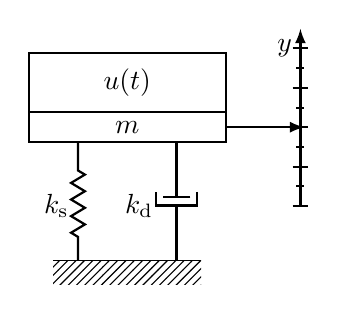
\begin{tikzpicture}[every node/.style={draw,outer sep=0pt,thick}]
    \tikzstyle{spring}=[thick,decorate,decoration={zigzag,pre length=0.3cm,post length=0.3cm,segment length=6}]
    \tikzstyle{damper}=[thick,decoration={markings,  
    mark connection node=dmp,
    mark=at position 0.5 with 
    {
    \node (dmp) [thick,inner sep=0pt,transform shape,rotate=-90,minimum width=15pt,minimum height=3pt,draw=none] {};
    \draw [thick] ($(dmp.north east)+(2pt,0)$) -- (dmp.south east) -- (dmp.south west) -- ($(dmp.north west)+(2pt,0)$);
    \draw [thick] ($(dmp.north)+(0,-5pt)$) -- ($(dmp.north)+(0,5pt)$);
    }
    }, decorate]
    \tikzstyle{ground}=[fill,pattern=north east lines,draw=none,minimum width=0.63cm,minimum height=0.3cm]

    \node (M) [minimum width=2.5cm,minimum height=0.05cm] {$m$};
    \node (Mu) [minimum width=2.5cm,minimum height=0.75cm,yshift=0.57cm] {$u(t)$};

    \node (ground1) at (M.south) [ground,yshift=-1.5cm,xshift=-0.625cm,anchor=north] {};
    \draw (ground1.north west) -- (ground1.north east);
    \draw [spring] (ground1.north) -- ($(M.south east)!(ground1.north)!(M.south west)$);

    \node (groundc) at (M.south) [ground,yshift=-1.5cm,anchor=north] {}; 
    \draw (groundc.north west) -- (groundc.north east);

    \node (ground2) at (M.south) [ground,yshift=-1.5cm,xshift=0.625cm,anchor=north] {};
    \draw (ground2.north west) -- (ground2.north east);
    \draw [damper] (ground2.north) -- ($(M.south east)!(ground2.north)!(M.south west)$);

    \node[draw=none,fill=none] at (-0.9cm,-1cm) {$k_{\mathrm{s}}$};
    \node[draw=none,fill=none] at (0.15cm,-1cm) {$k_{\mathrm{d}}$};
    \node[draw=none,fill=none] at (2.0cm,1.0cm) {$y$};
    \draw [-latex,thick]  ++(2.2cm,-1cm) -- +(0cm,2.25cm);

    \draw [-latex,thick] (M.east) ++(0,0) -- +(1cm,0);
    \draw [line width=0.25mm] (2.2cm,-1cm) -- (2.2cm,1cm);
    \draw [line width=0.25mm] (2.1cm,-1cm) -- (2.3cm,-1cm);
    \draw [line width=0.25mm] (2.1cm,1cm) -- (2.3cm,1cm);
    \draw [line width=0.25mm] (2.1cm,-0.5cm) -- (2.3cm,-0.5cm);
    \draw [line width=0.25mm] (2.1cm,0.5cm) -- (2.3cm,0.5cm);
    \draw [line width=0.25mm] (2.15cm,-0.25cm) -- (2.25cm,-0.25cm);
    \draw [line width=0.25mm] (2.15cm,0.25cm) -- (2.25cm,0.25cm);
    \draw [line width=0.25mm] (2.15cm,-0.75cm) -- (2.25cm,-0.75cm);
    \draw [line width=0.25mm] (2.15cm,0.75cm) -- (2.25cm,0.75cm);
    \draw [line width=0.25mm] (2.1cm,0cm) -- (2.3cm,0cm);

    \end{tikzpicture}

    \caption{\label{fig:simple_msd_system}  \color{blue} A second order mass-spring-damper model represents the weighing sensor. The application of the mass $u$ causes a change in the position $y$ of the scale. \color{black} } 
    \end{figure}


    \renewcommand{\thefigure}{2.2}
    \begin{figure}[!htbp]
    \centering
    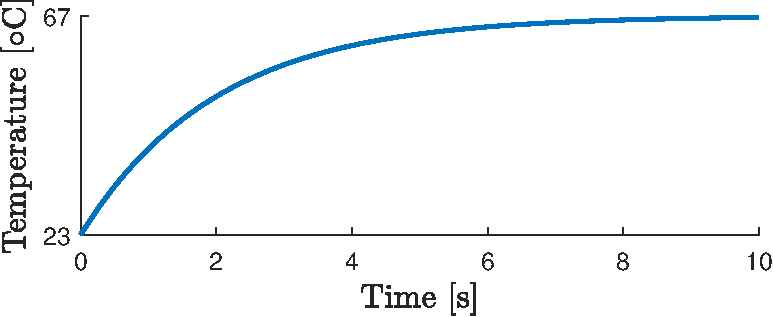
\includegraphics[width=0.6\columnwidth]{../ChapterIntroduction/fig/Fig_2.pdf} 
    \caption{ \label{fig:thermometer} 
    \color{blue} This simulation shows an example of the temperature change experimented by a thermometer, with $k_T=0.5 s^{-1}$, caused by applying a step input of 67 $\circ \mathrm{C}$  when the thermometer was initially at 23 $\circ \mathrm{C}$. In this example, we should wait 10 s to have an estimation of the input with a relative error lower than 0.5\%. \color{black} }
    \end{figure}

    \renewcommand{\thefigure}{2.3}
    \begin{figure}[!htbp]
    \centering
    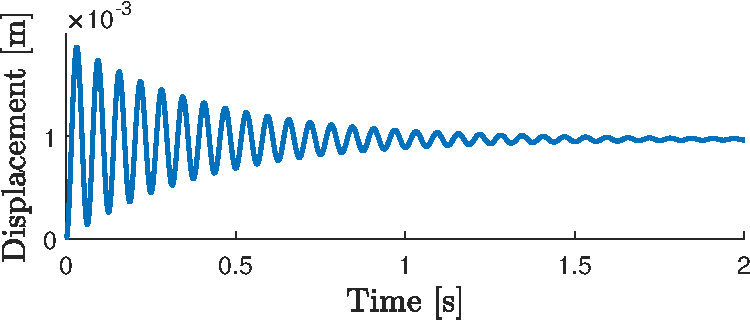
\includegraphics[width=0.6\columnwidth]{../ChapterIntroduction/fig/Fig_3.pdf} 
    \caption{ \label{fig:scale} 
    \color{blue} This simulation illustrates the displacement observed when a constant input $u=1 \mathrm{kg}$ is applied to a weighing sensor in equilibrium. The sensor parameters are $k_{\mathrm{d}} = 5 \mathrm{N s/m}$, and $k_{\mathrm{s}} = 10000 \mathrm{N/m}$. In this conditions, the user has to wait more that 2 s to observe a stabilization on the scale and to estimate the mass from reading the final value of the displacement with a relative error smaller than 0.72\%. \color{black}  }
    \end{figure}

    \color{black}

    
    \end{itemize}
    \item Detailed remarks:
    
    {\bfseries The detailed remarks in this list have been attended accordingly: }
    
    \begin{itemize}
    \item Citations that are used in-line should have brackets only around the year, not around the authors’ names. For instance on page 3, line -2 is written “reviewed in [Hack and ten Caten, 2012]”. This should be displayed as “reviewed in Hack and ten Caten [2012]. In LaTeX this can typically be done by making the proper distinction between the commands \ citet and \ citep. The former is used for references in text, the latter for parenthetical references.
    \item  On page 1 of the PDF (front of thesis), I believe also N. Deligiannis should be mentioned with the title “prof.”. 
    \item Page 1 of thesis: typo on line 6: “and on the sensor initial conditions” => “sensor’s initial conditions”
    \item Page 3, line -2: “uncertainty analysis are reviewed” => “is reviewed”
    \item Page 3, line -1: remove comma before “that”
    \item Page 3, line -2: fix the in-text reference (see above)
    \item Page 4, lines 11-13: fix the in-text references (see above)
    \item Page 5, line 5: Remove “The” at the beginning of the sentence (The Hankel…)
    \item Page 6, line 10: fix the in-text references (see above)
    \item Page 7, lines 10-11: the sentence on heart and breathing physiological monitoring sounds a bit awkward. Please reformulate.
    \item Page 9, line -1: fix the in-line reference (see above)
    \item Page 10, lines 1-3: in the enumeration of the types of sensors, remove the article ‘the’ before the sensor name. So: “like three-axis sensors [ref], radio-frequency intruder sensors [ref], and radar sensors [ref]. 
    \item Page 10, equation 3.10: The symbol D was not bold in the equations above. Be consistent!
    \item Page 10, caption of figure: replace “reverts” by “inverts”
    \item Page 11, line 9, put “poles” between parentheses instead of between commas.
    \item Page 12, line -6: “that in matrix form is” => “which in matrix form is”
    \item Page 13, line -9: “in the practice” => “in practice”
    \item Page 14, line -14: missing space between “problem” and “(3.11)”
    \item Page 16, halfway page: the sentence “Applying a second-order…” is not a proper sentence (perhaps fix this by removing “that”).
    \item Page 16 introduces seemingly some new notation, e.g., b(.), mu(.) and C(.). While their meaning is clear from the context, it is desirable to give proper definitions when introducing new mathematical tools.
    \item Page 17, line -1: fix in-text references (see above)
    \item Page 20 (and beyond): The abbreviation CRLB is introduced, but sometimes CRB is used instead.
    \item Page 21, line -10: fix in-text reference (See above)
    \item Page 35, second sentence “The sensor is a dynamic…” is not a proper sentence.
    \item Page 50: Try to reorganize this section into two or more paragraphs.
    \item Page 59, line 2: fix in-text reference (See above)
    \item Page 74, line 11: “The learning obtained from…” this is an awkward sentence; please reformulate
    \item Page 81, all three journal publication references do not have (or have wrong?) page numbers.
    \end{itemize}
\end{itemize}



\bibliography{../Gus-thesis.bib}


\end{document}
